\documentclass[11pt,a4paper]{article}

% ------------------------------------------------------------------
%  Packages
% ------------------------------------------------------------------
\usepackage[utf8]{inputenc}
\usepackage[T1]{fontenc}
\usepackage[english]{babel}
\usepackage{amsmath,amssymb}
\usepackage{graphicx}
\usepackage{siunitx}
\usepackage{booktabs}
\usepackage{caption}
\usepackage{subcaption}
\usepackage[hidelinks]{hyperref}
\usepackage{geometry}
\geometry{margin=2.5cm}
\usepackage{physics}
\usepackage{float}

\graphicspath{{figures/}}

\sisetup{
    separate-uncertainty = true,
    per-mode = symbol,
}

% ------------------------------------------------------------------
%  Title
% ------------------------------------------------------------------
\title{%
    \vspace{-1.0cm}
    {\large University of Leipzig}\\[0.2cm]
    {\normalsize Advanced Physics Laboratory}\\[1.5cm]
    {\Huge \bfseries Digital RF-Receiving Technique\\[0.3cm] and Electron-Paramagnetic\\[0.3cm] Resonance (EPR)}\\[1.0cm]
}

\author{%
    % TODO: Namen und Matrikelnummern eintragen
    \begin{tabular}{c}
        Fynn Kanja \\
        % Matrikelnummer
    \end{tabular}
}

\date{Experiment No.~5 \\[0.2cm] Leipzig, \today}

% ------------------------------------------------------------------
\begin{document}

\maketitle
\thispagestyle{empty}
\newpage

\tableofcontents
\newpage

% ==================================================================
\section{Theoretical Background}
% ==================================================================

\subsection{Electron Paramagnetic Resonance (EPR)}
Electron paramagnetic resonance (EPR), also known as electron spin resonance
(ESR), is a spectroscopic method used to study materials that contain
\emph{unpaired electrons}. The paramagnetic sample is placed in a static
magnetic field and irradiated with microwaves (GHz range). The microwave field
interacts with the magnetic moments of the unpaired electrons, and from the
resulting resonance one can obtain information about the structure and the
dynamics of the substance. EPR is closely related to nuclear magnetic resonance
(NMR); however, NMR addresses nuclei with non-zero spin, whereas EPR addresses
the spins of unpaired electrons.

\subsection{Zeeman Effect}
An electron carries an intrinsic spin and an associated magnetic moment. When an
external magnetic field $B$ is applied to a paramagnetic substance, the spin of
an unpaired electron can align either parallel or anti-parallel to the field,
corresponding to the spin states $m_s = \pm\tfrac{1}{2}$. These two orientations
have different energies, so the field lifts the degeneracy of the electron spin
states. This splitting is known as the \emph{Zeeman effect}
(see Figure~\ref{fig:zeeman}). The energy difference between the two levels is

\begin{equation}
    \Delta E = g\,\mu_B\,B ,
    \label{eq:zeeman}
\end{equation}

where $B$ is the external magnetic flux density, $\mu_B$ is the Bohr magneton and
$g$ is the Land\'e $g$-factor, which relates the magnetic moment to the angular
momentum of the electron system. For a free electron $g = 2.0023$.

\begin{figure}[H]
    \centering
    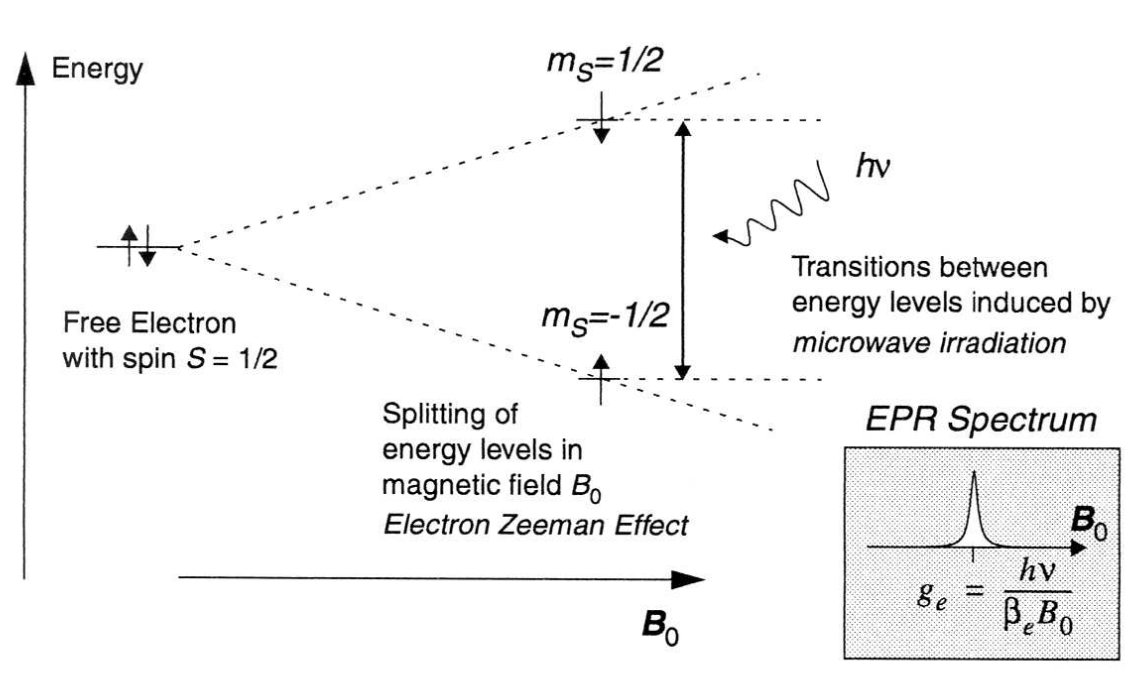
\includegraphics[width=0.65\textwidth]{zeeman_splitting.png}
    \caption{Zeeman splitting of the spin states of a free electron in an
             external magnetic field $B_0$: the degenerate $m_s = \pm 1/2$
             levels split linearly with $B_0$, and microwave irradiation of
             frequency $\nu$ drives transitions between them once
             $h\nu = g\mu_B B_0$.}
    \label{fig:zeeman}
\end{figure}

\subsection{Resonance Condition}
An unpaired electron can change its spin state by absorbing or emitting a photon
whose energy equals the level splitting, $h\nu = \Delta E$. Combining this with
Equation~\eqref{eq:zeeman} yields the fundamental equation of EPR spectroscopy,

\begin{equation}
    h\nu_0 = g\,\mu_B\,B_0 ,
    \label{eq:resonance}
\end{equation}

where $h$ is the Planck constant, $\nu_0$ the frequency of the high-frequency
alternating ($B_1$) field, and $B_0$ the static magnetic flux density required
for resonance. The $B_1$ field is oriented perpendicular to $B_0$. Solving
Equation~\eqref{eq:resonance} for the $g$-factor gives the relation used in the
evaluation of the measurements,

\begin{equation}
    g = \frac{h\,\nu_0}{\mu_B\,B_0} .
    \label{eq:gfactor}
\end{equation}

\subsection{EPR Spectrum}
The majority of EPR measurements are performed in the microwave range of
\SIrange{9}{10}{\giga\hertz} (X-band), with resonance fields of approximately
\SI{0.35}{\tesla}. In principle a spectrum can be obtained either by sweeping
the microwave frequency at constant field or by sweeping the magnetic field at
constant frequency. In practice the frequency is usually kept fixed and the
field is swept through the resonance condition. Because the lower energy level is
slightly more populated according to the Boltzmann distribution, there is a net
absorption of microwave power at resonance. The detected EPR spectrum is commonly
the first derivative of this absorption line (Figure~\ref{fig:epr-spectrum});
in the present experiment the \emph{dispersion} signal of the resonance is
recorded (the characteristic S-shaped frequency shift of the down-converted
signal across resonance).

\begin{figure}[H]
    \centering
    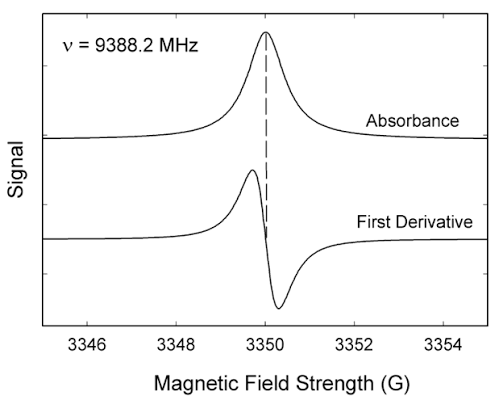
\includegraphics[width=0.55\textwidth]{epr_spectrum.png}
    \caption{Typical EPR absorption line and its first derivative, the
             commonly recorded EPR spectrum.}
    \label{fig:epr-spectrum}
\end{figure}

\subsection{Radio-Frequency Techniques}
Since EPR uses radiation in the GHz range, it is useful to understand the
RF techniques employed to generate and detect such signals. The two most
relevant techniques for this experiment are frequency modulation and frequency
mixing.

\subsubsection{Frequency Modulation}
Modulation is an RF technique in which a periodic carrier waveform is altered by a
second (modulation) waveform. In frequency modulation the instantaneous
frequency of the carrier is varied according to the modulation signal. This
technique is fundamental to radio communication, as it allows a single carrier to
be separated from other signals in the spectrum.

\begin{figure}[H]
    \centering
    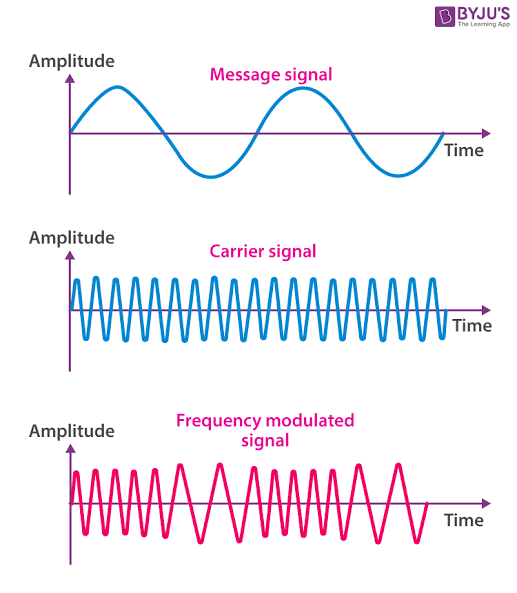
\includegraphics[width=0.55\textwidth]{frequency_modulation.png}
    \caption{Frequency modulation: the instantaneous frequency of the carrier
             signal is varied according to the message signal.}
    \label{fig:fm-principle}
\end{figure}

\subsubsection{Frequency Mixing}
Frequency mixing is a process in which two signals of frequencies $f_1$ and $f_2$
are combined in a (nonlinear) mixer. At the output, new signals appear at the
sum and difference frequencies,

\begin{equation}
    f_{\pm} = f_1 \pm f_2 ,
    \label{eq:mixing}
\end{equation}

in addition to the original frequencies. In a real mixer higher-order
combinations such as $f_1 \pm 2f_2$ may also appear. Mixing is the working
principle of the low-noise block (LNB) used to down-convert the GHz EPR signal
into the easily measurable range of a few hundred MHz (see
Section~\ref{sec:lnb}).

\begin{figure}[H]
    \centering
    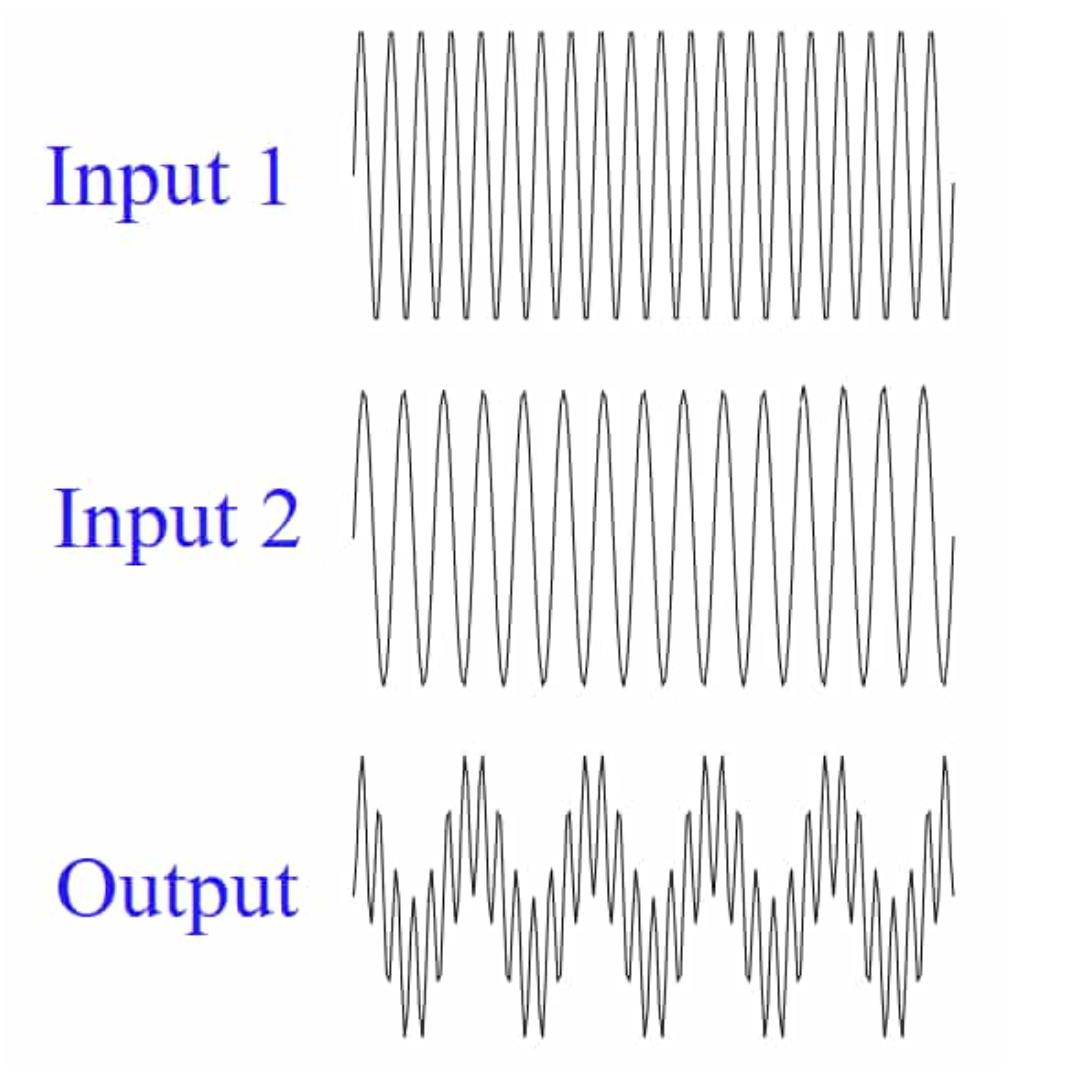
\includegraphics[width=0.35\textwidth]{signal_mixing.png}
    \caption{Mixing two sine waves: the mixer output contains the sum and
             difference frequencies of the two inputs.}
    \label{fig:mixing-principle}
\end{figure}

\subsection{Materials}
EPR is sensitive to substances containing unpaired electrons, in particular
\begin{itemize}
    \item free radicals in solids, liquids or gases, and
    \item paramagnetic transition-metal ions.
\end{itemize}
In this experiment DPPH and Ultramarine were used as samples at different
concentrations / dilution levels.

\subsubsection{DPPH}
Diphenyl-Picryl-Hydrazyl (DPPH) is a stable organic radical and a standard
reference material for EPR. It is a dark crystalline powder with one unpaired
electron, delocalised over the hydrazyl nitrogen and the picryl ring
(Figure~\ref{fig:dpph-structure}). Its $g$-factor is $g = 2.0036$, very close
to that of the free electron, which makes it a convenient calibration
standard.

\begin{figure}[H]
    \centering
    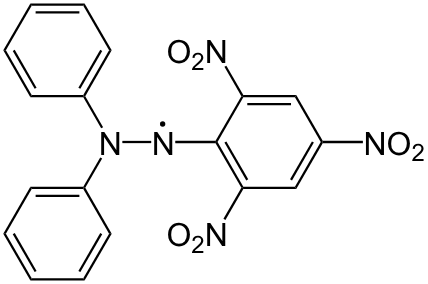
\includegraphics[width=0.45\textwidth]{dpph_structure.png}
    \caption{Structural formula of DPPH; the unpaired electron is delocalised
             over the hydrazyl nitrogen and the picryl ring.}
    \label{fig:dpph-structure}
\end{figure}

\subsubsection{Ultramarine}
Ultramarine (UM) is another commonly used EPR substance owing to its strong
paramagnetic character, which arises from sulfur radicals whose detailed
structure is largely unknown. Its chemical formula is
$\mathrm{Na_{8-10}Al_{6}Si_{6}O_{24}S_{2-4}}$. Its $g$-factor of $g = 2.0290$
differs noticeably from that of the free electron ($g = 2.0023$).

% ==================================================================
\section{Experimental Set-up and Methodology}
% ==================================================================
In an EPR measurement the absorption (here: dispersion) of microwaves by the
sample is recorded as a function of a slowly varying magnetic field, while the
microwave frequency is kept constant. Figure~\ref{fig:system-block} gives an
overview of a classical EPR spectrometer; the main components of the set-up
are described below.

\begin{figure}[H]
    \centering
    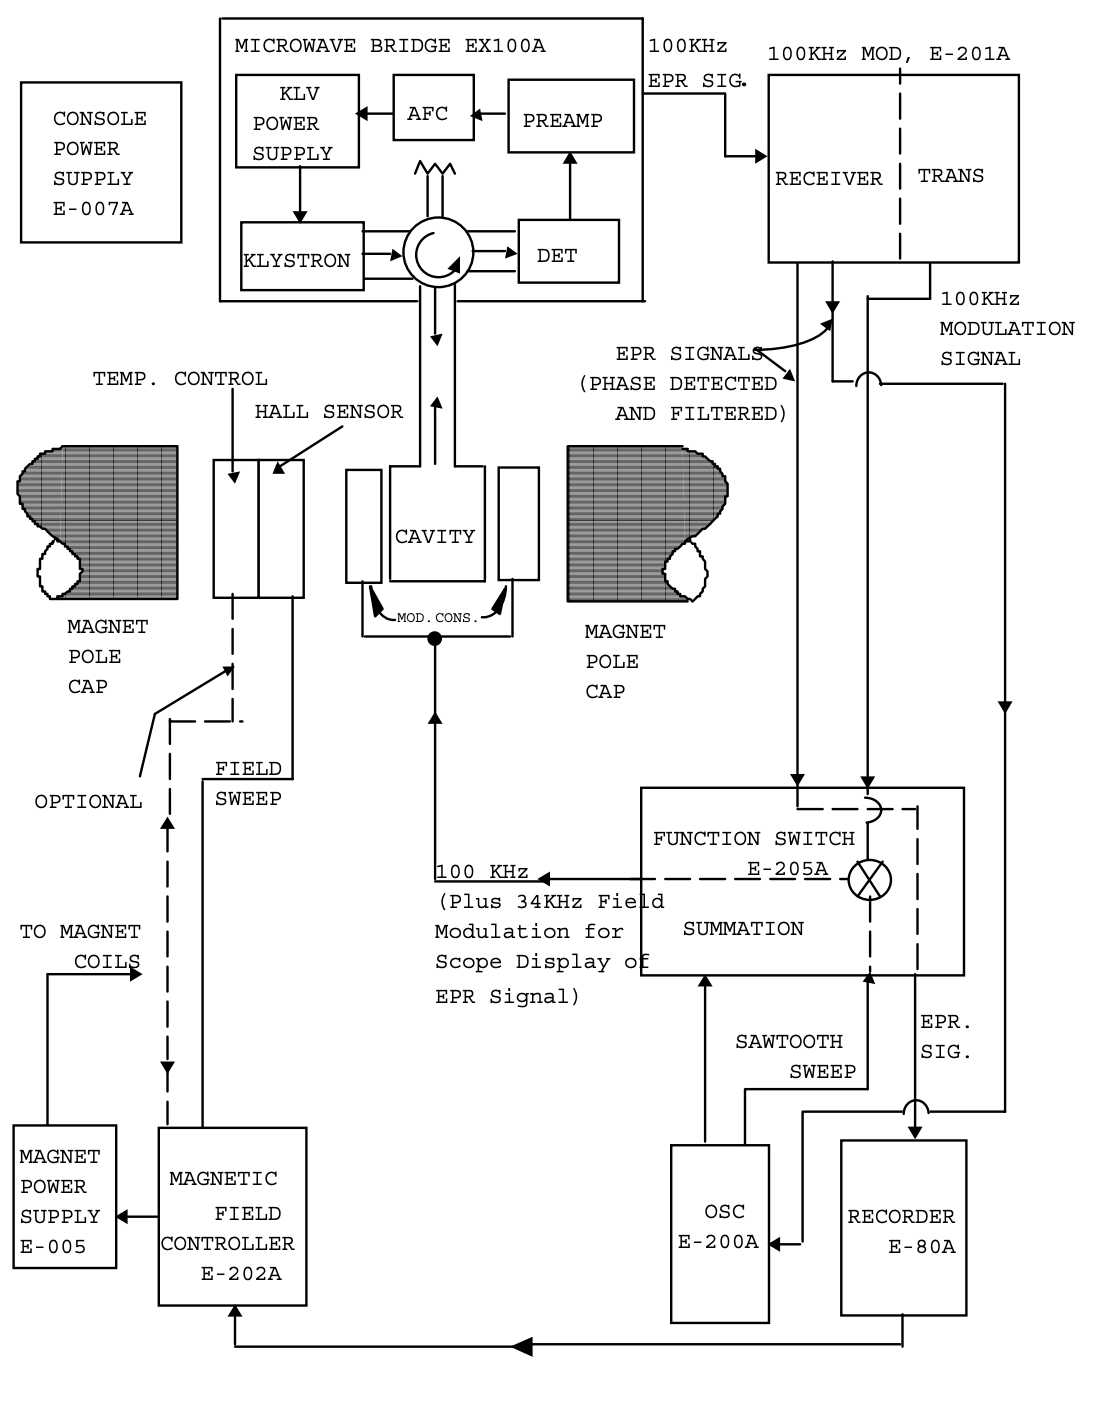
\includegraphics[width=0.7\textwidth]{epr_system_block_diagram.png}
    \caption{Block diagram of a classical EPR spectrometer: the microwave
             bridge, the sample cavity between the magnet pole caps, the
             field sweep / modulation electronics and the signal-recovery
             chain.}
    \label{fig:system-block}
\end{figure}

\subsection{Signal Sources and Mixing Stage}
For the RF mixing and modulation experiments both channels of the RIGOL
Dual-Channel Arbitrary / Waveform Generator DG1022 were used as signal sources.
The signals were combined in a Hewlett-Packard Model 10514A double-balanced
mixer. To protect the mixer, no more than \SI{40}{\milli\ampere} may flow into
any of its ports, and the power in the \SI{50}{\ohm} system was always kept below
\SI{5}{\milli\watt} (corresponding to a maximum of about \SI{1.4}{V_{pp}} or
\SI{0.5}{V_{rms}}). The input signals and the mixed output $X$ were observed in
the time domain with the TiePie Handyscope HS3 (used as a two-channel
oscilloscope) and an analog oscilloscope, while the spectral content was measured
with the SDRplay RSP1 radio spectrum processor in combination with the HDSDR
software. A PRL~T5075 attenuator ($\geq \SI{-60}{\decibel}$ for mixing,
$\geq \SI{40}{\decibel}$ for antenna reception) protected the RSP1 input.

\begin{figure}[H]
    \centering
    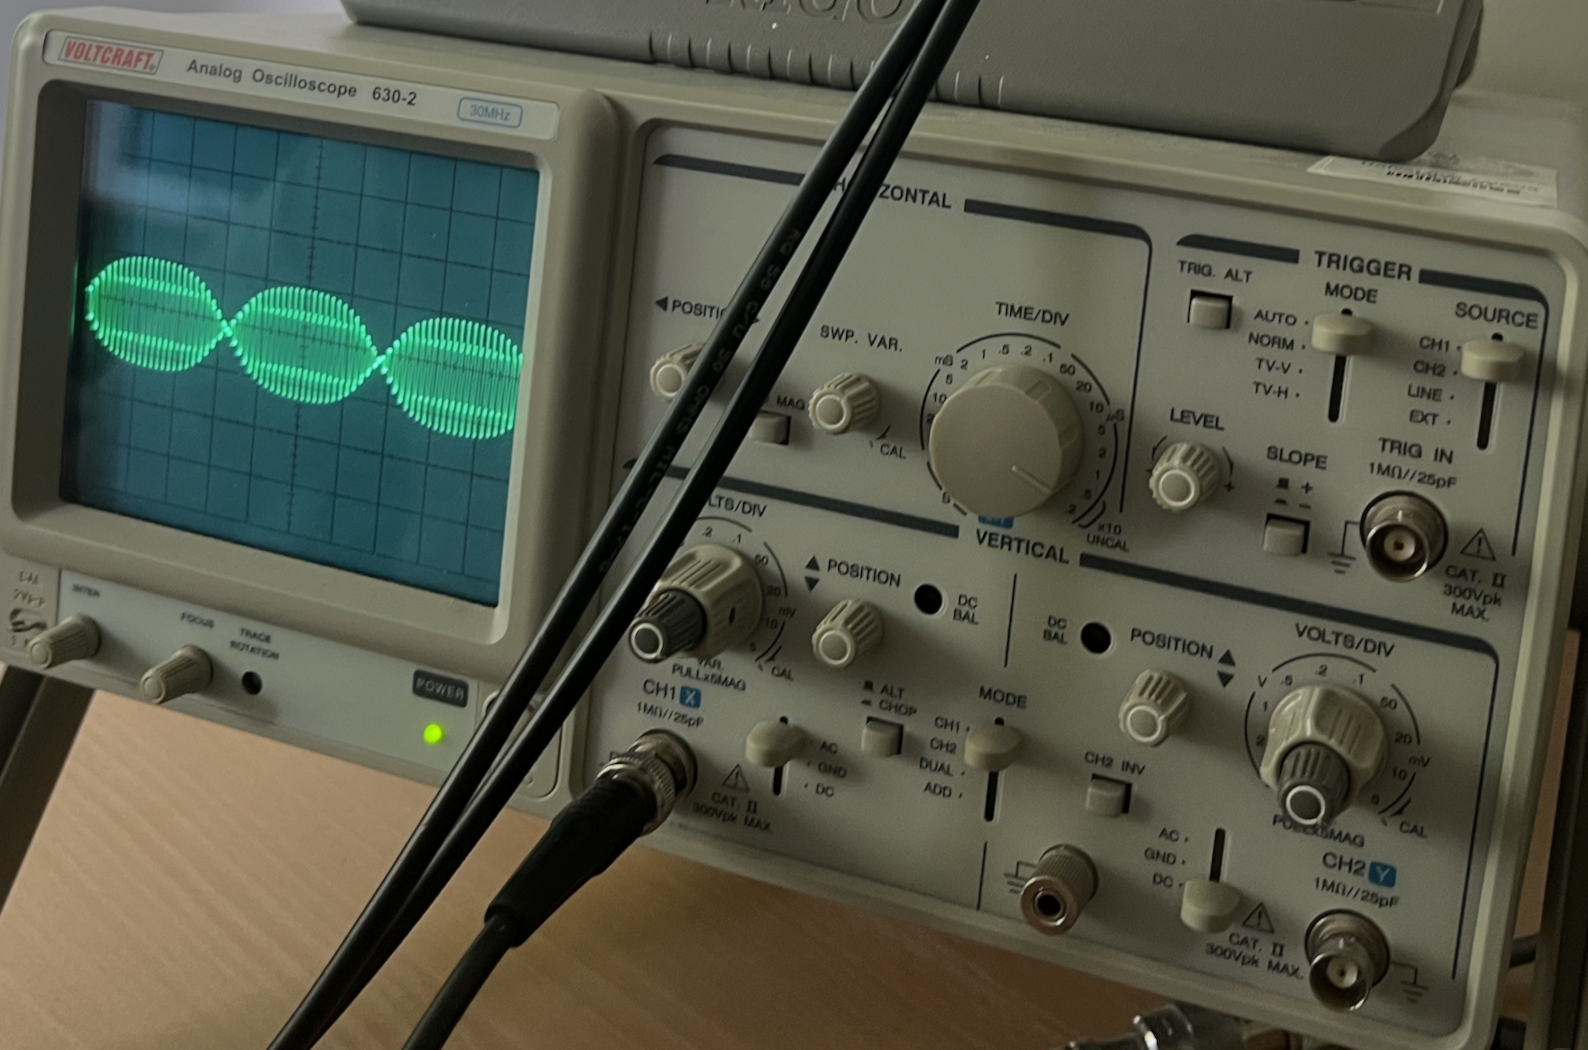
\includegraphics[width=0.5\textwidth]{setup_mixing_scope.png}
    \caption{Analog oscilloscope display of the mixed output $X$: the
             amplitude-modulated beat waveform of the two mixed DG1022
             signals.}
    \label{fig:setup-scope}
\end{figure}

\subsection{Microwave Bridge and Magnet System}
In a classical EPR spectrometer the microwave bridge generates the microwaves
(e.g.\ with a klystron) and detects the reflected EPR signal via a circulator
and a detector diode (Figure~\ref{fig:bridge}). The sample sits in a high-$Q$
resonant cavity, defined by
$Q = \omega \cdot (\text{energy stored}) / (\text{power dissipated})$, which is
surrounded by a pair of magnet pole pieces / Helmholtz coils. The sample is
placed at the position of maximum $B_1$ field and perpendicular to the static
field $B_0$. Because the linearly polarised $B_1$ field can be decomposed into
two counter-rotating circular components, only the component co-rotating with the
electron precession drives the resonance transitions.

\begin{figure}[H]
    \centering
    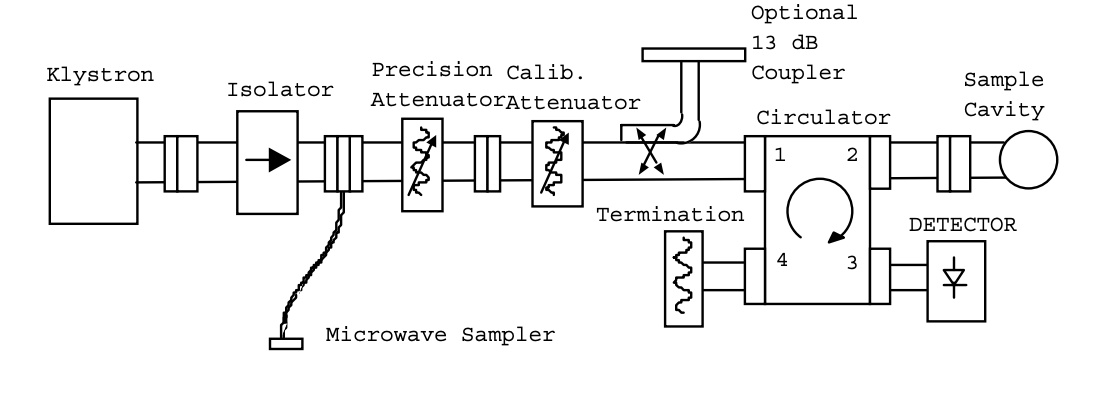
\includegraphics[width=0.9\textwidth]{microwave_bridge_schematic.png}
    \caption{Schematic of a microwave bridge: klystron, isolator, precision
             and calibrated attenuators, circulator and sample cavity, with
             the reflected signal directed to the detector.}
    \label{fig:bridge}
\end{figure}

\subsection{Magnetic Field Sweep}
\label{sec:sweep}
The static magnetic flux density is set by the output voltage of the power
supply and is displayed in millitesla. The field is swept through the resonance
by a programmed voltage sequence on the controlling notebook. The sequence used here had the
following parameters:
\begin{itemize}
    \item start voltage: \SI{26}{\volt};
    \item one step per second (\SI{1}{\second} per segment);
    \item voltage increment per step: \SI{0.05}{\volt};
    \item number of steps: 81;
    \item the final step resets the supply to \SI{10}{\volt}.
\end{itemize}
Before starting the sequence, the voltage is manually set close to the first
value of the file. From this sequence the field gradient (in \si{Gs/s}) can be
determined.

\subsubsection{Magnetic Field Calibration}
\label{sec:calibration}
To convert the operating point of the power supply into the actual magnetic flux
density $B_0$, a calibration data set was recorded from the supplementary video.
For each step of the sweep, the supply voltage $U$, the coil current $I$ and the
field $B_0$ displayed by the Hall sensor (in \si{\milli\tesla}) were read off,
yielding 81 data points.

A first inspection shows that the \emph{voltage} is not a suitable control
variable: above $U \approx \SI{26}{\volt}$ the supply runs into its voltage
limit, so $U$ saturates while the current and the field keep rising. A fit of
$B_0$ against $U$ is correspondingly poor ($R^2 \approx 0.77$). This is expected
physically, since the field of the electromagnet is set by the \emph{coil
current}, not by the supply voltage. We therefore calibrate $B_0$ against the
current $I$:

\begin{equation}
    B_0(I) = a\,I + b ,
    \label{eq:cal}
\end{equation}

A linear least-squares fit (Figure~\ref{fig:cal}) gives

\begin{align}
    a &= \SI{99.6(14)}{\milli\tesla\per\ampere}, &
    b &= \SI{-11.5(53)}{\milli\tesla}, &
    R^2 &= 0.985 .
\end{align}

The first four points (supply settling, before the current has stabilised at
the start of the ramp) and one obvious read-off error in the current column
were excluded from the fit (open circles in Figure~\ref{fig:cal}). The high
$R^2$ confirms the expected linear relation
between coil current and field. Equation~\eqref{eq:cal} is used to assign a
magnetic flux density to every point of the recorded dispersion curves; the
covered range $I = \SIrange{3.1}{4.0}{\ampere}$ corresponds to
$B_0 \approx \SIrange{287}{383}{\milli\tesla}$, which brackets the expected DPPH
resonance field of $\approx \SI{0.38}{\tesla}$.

For the point-by-point conversion of the recorded dispersion sweeps, however,
only the \emph{programmed supply voltage} is known for every data point (the
coil current was not logged alongside the dispersion measurement). Each sweep
follows the fixed voltage sequence of Section~\ref{sec:sweep}
(\SI{26}{\volt} start, \SI{0.05}{\volt} per one-second step), so every sample
can be assigned a nominal voltage $U(t)$. The magnetic field for that voltage
is then obtained by piecewise-linear interpolation of the tabulated
$(U, B_0)$ pairs from the calibration video (the same data set as above,
restricted to $U \geq \SI{26}{\volt}$ to remove the settling transient) rather
than the global current-based fit: since the calibration was recorded on the
same \SI{0.05}{\volt} grid as the sweep sequence, direct interpolation avoids
the residual scatter of a single straight-line fit and reproduces the local
curvature of $B_0(U)$ visible in Figure~\ref{fig:cal}. The last sweep step
(\SI{30}{\volt}) lies \SI{0.05}{\volt} beyond the calibrated range and is
obtained by linear extrapolation from the last two calibration points.

\begin{figure}[H]
    \centering
    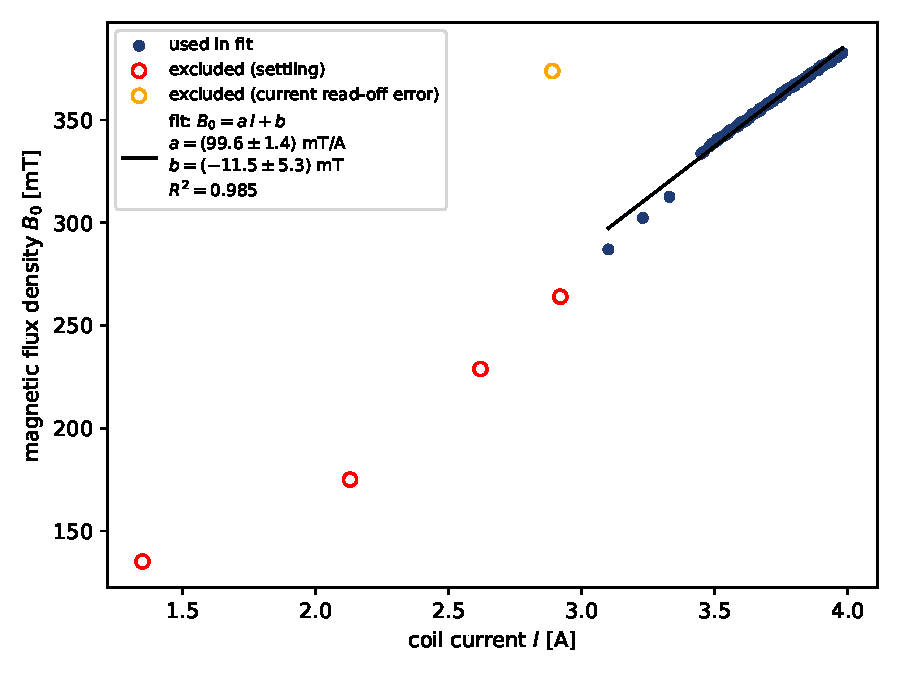
\includegraphics[width=0.68\textwidth]{calibration_fit.pdf}
    \caption{Magnet calibration: displayed magnetic flux density $B_0$ versus
             coil current $I$, with the linear fit
             $B_0 = a\,I + b$ (Equation~\eqref{eq:cal}). Open circles mark
             points excluded from the fit (red: initial supply settling;
             orange: current read-off error).}
    \label{fig:cal}
\end{figure}

\subsection{Low-Noise Block (LNB)}
\label{sec:lnb}
The EPR signal of the DPPH and Ultramarine samples is detected with a modified
satellite low-noise block (LNB) ``OSLSO''. It contains two local oscillators
(LO) operating simultaneously at \SI{9.75}{\giga\hertz} and
\SI{10.6}{\giga\hertz}. The sample is coupled to the dielectric resonator (DR,
the small violet ring cylinder) at the \SI{10.6}{\giga\hertz} frequency. By
mixing the two LO frequencies (Equation~\eqref{eq:mixing}) and down-converting,
the dispersion signal of the resonance is shifted to the easily measurable region
around \SI{800}{\mega\hertz} at the LNB output, where it is recorded with the
RSP1 / HDSDR system. For Task~6 a calibrated PLL LNB with a single, exactly known
LO frequency of \SI{9.75}{\giga\hertz} is used instead.

\subsection{Data Processing}
\label{sec:processing}
For Tasks~4--6 the HDSDR waterfall / spectrum display was photographed during
the field sweep (rather than exported as a screenshot). Each photograph was
then digitised manually with \texttt{WebPlotDigitizer}: the frequency ruler
of the waterfall gives the calibration for the output frequency $\nu$, and
the timestamp labels running along the waterfall give the calibration for
elapsed real time, so every clicked point on the dispersion trace yields a
$(\nu, t)$ pair with $t$ the wall-clock time at which that frequency was
observed.

The elapsed time $t$ is then converted to the corresponding supply voltage
$U(t)$ using the fact that the voltage sequence is known exactly
(Section~\ref{sec:sweep}): counting back from the last digitised point of
each measurement, the sweep covers the final \SI{80}{\second} of the
\SI{81}{}-step sequence, rising linearly from \SI{26}{\volt} to
\SI{30}{\volt} at \SI{0.05}{\volt} per one-second step. Duplicate points
digitised within the same one-second voltage step are averaged. The voltage
$U(t)$ is finally converted to the magnetic flux density $B_0$ by
interpolating the tabulated calibration curve from the supplementary video
(Section~\ref{sec:calibration}), giving the same $\nu$ versus $B_0$
representation as a direct digitisation of the field axis would.

The raw frequency trace still carries a slow drift across the sweep on top of
the S-shaped dispersion feature, most visible for the weakly paramagnetic
samples; this drift is removed with a wide rolling-median baseline, and the
resonance field $B_0$ is read off at the point of steepest slope of the
\emph{residual} (measured $-$ baseline), i.e.\ the inflection / zero crossing
of the S-shaped feature itself. $B_0$ is then inserted into
Equation~\eqref{eq:gfactor}, together with the nominal LNB coupling frequency
($\nu_0 = \SI{10.6}{\giga\hertz}$ for Tasks~4/5, Section~\ref{sec:lnb}; the
exactly known $\nu_0 = \SI{9.75}{\giga\hertz}$ of the calibrated PLL LNB for
Task~6), to determine the $g$-factor.

% ==================================================================
\section{Measurements and Analysis}
% ==================================================================
\textit{Hinweis: Für Task~4--6 wurden die im Labor fotografierten
Dispersionskurven mit \texttt{WebPlotDigitizer} manuell digitalisiert, die
digitalisierte Zeit anhand der bekannten Spannungs-Sequenz (26--30\,V in
80\,s, Abschnitt~\ref{sec:sweep}) in eine Spannung umgerechnet und diese
Spannung mit der Kalibrierung aus Abschnitt~\ref{sec:calibration} in
Frequenz vs.\ Magnetfeld $B_0$ umgerechnet. Das Resonanzfeld $B_0$ wird an
der Stelle der steilsten Steigung der S-förmigen Dispersionskurve bestimmt
(Abschnitt~\ref{sec:processing}).}

% ------------------------------------------------------------------
\subsection{Task 1 -- Frequency Mixing and Modulation}
% ------------------------------------------------------------------
One channel of the DG1022 supplied a \SI{10}{\mega\hertz} sine wave at
\SI{0.5}{V_{rms}} (\SI{5}{\milli\watt}) to input~$L$ of the mixer; the second
channel supplied input~$R$ with a \SI{200}{\kilo\hertz} sine wave at
\SI{1}{\milli\watt} (\SI{0.22}{V_{rms}}). The mixed output was observed in the
time domain (Figure~\ref{fig:setup-scope}) and in the spectral domain with HDSDR
(Figure~\ref{fig:task1}). As expected from Equation~\eqref{eq:mixing}, sum and
difference signals appear symmetrically around the carrier; varying the second
frequency shifts the sidebands accordingly, and higher-order mixing products
($f_1 \pm 2f_2$, \dots) are visible as additional lines.

\begin{figure}[H]
    \centering
    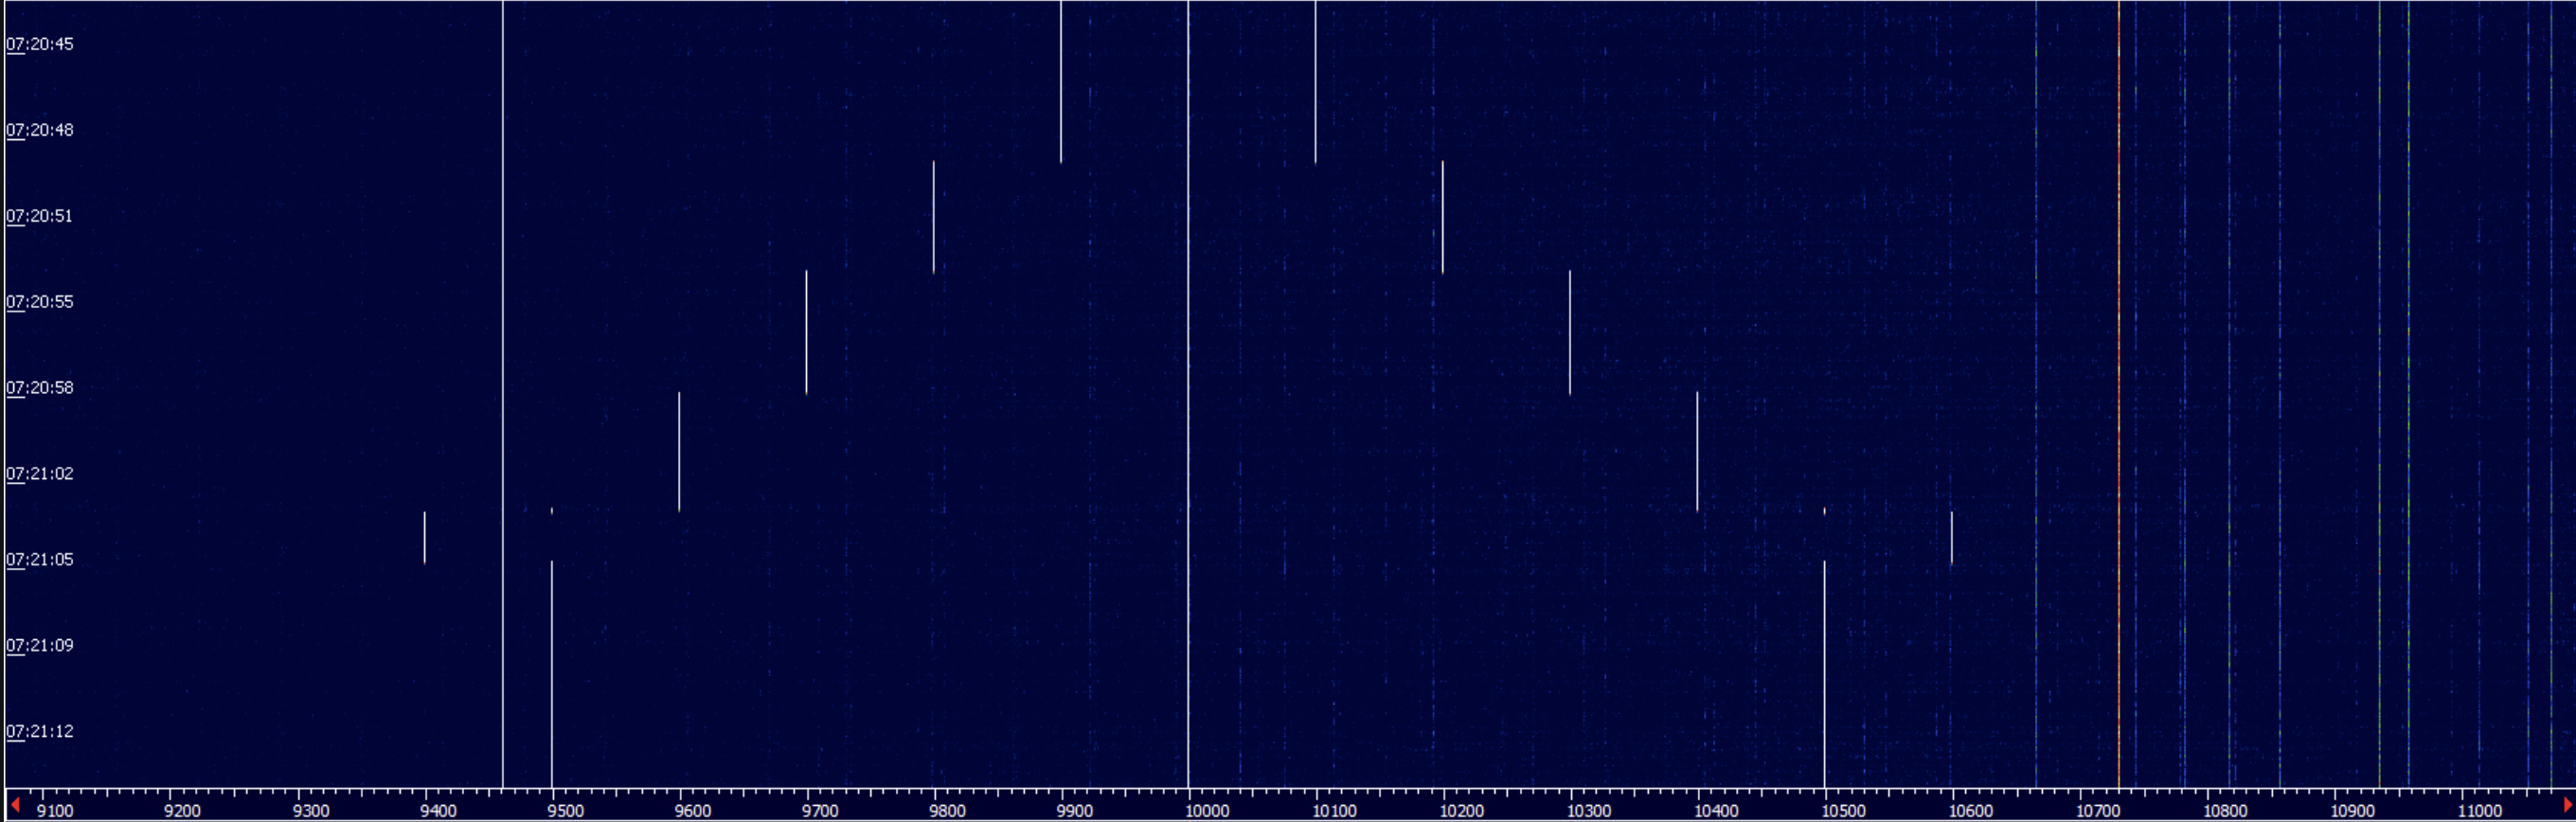
\includegraphics[width=0.85\textwidth]{task1_10mhz_hdsdr.png}
    \caption{HDSDR waterfall of the \SI{10}{\mega\hertz} mixing signal: as the
             second frequency $f_2$ was stepped, the sum/difference sidebands
             visibly jump to new positions. % TODO: Seitenbänder markieren
            }
    \label{fig:task1}
\end{figure}

% ------------------------------------------------------------------
\subsection{Task 2/3 -- Reception of VLF, FM and PMR Signals}
% ------------------------------------------------------------------
Using the laboratory antennas (active VLF antenna and VHF/FM wire antenna) and
the RSP1/HDSDR receiver, signals in different bands were received and analysed.
Figure~\ref{fig:fm} shows the FM broadcast band (local stations,
e.g.\ \emph{Radio Sachsen} / \emph{Energy Sachsen}), and
Figure~\ref{fig:pmr} shows a walkie-talkie stepping through channels 1--8,
spanning roughly \SIrange{441.46}{441.84}{\mega\hertz}. % TODO: genaue
% Kanalfrequenzen, Kanalabstand, Bandbreite und Modulationsart bestimmen;
% DCF77 / EFR (DCF49, DCF39, HGA22) im VLF-Bereich ergänzen.

\begin{figure}[H]
    \centering
    \begin{subfigure}{0.48\textwidth}
        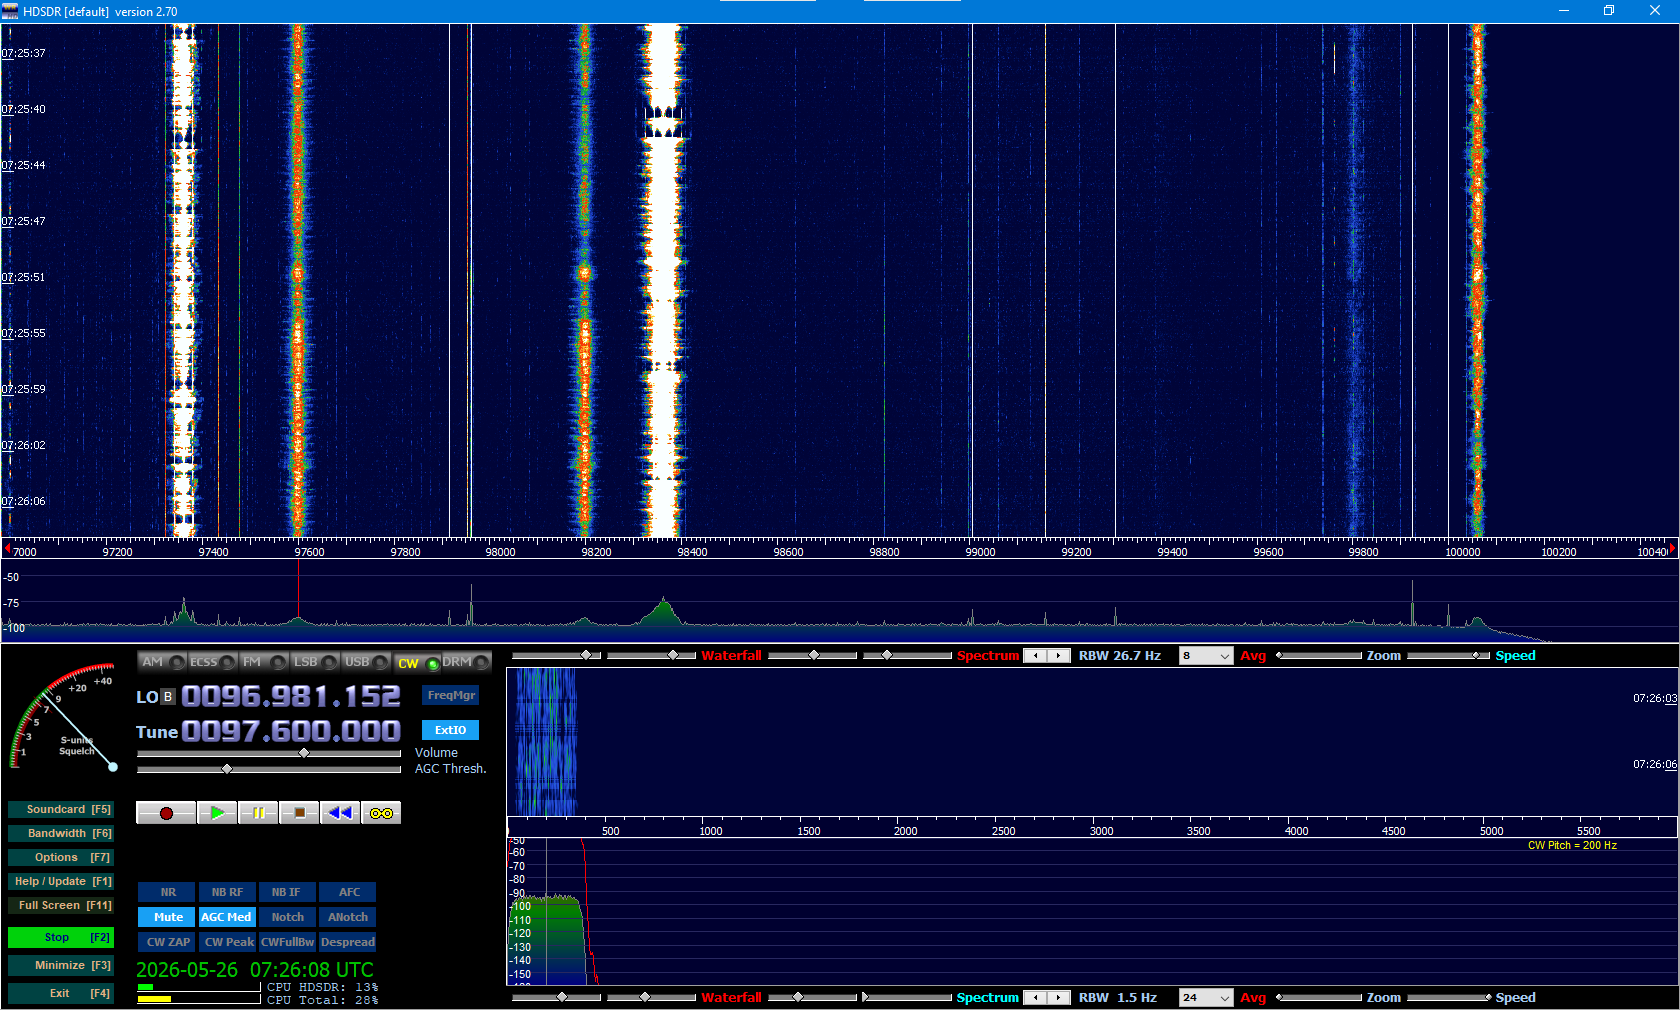
\includegraphics[width=\textwidth]{task3_fm_radio.png}
        \caption{FM broadcast band.}
        \label{fig:fm}
    \end{subfigure}\hfill
    \begin{subfigure}{0.48\textwidth}
        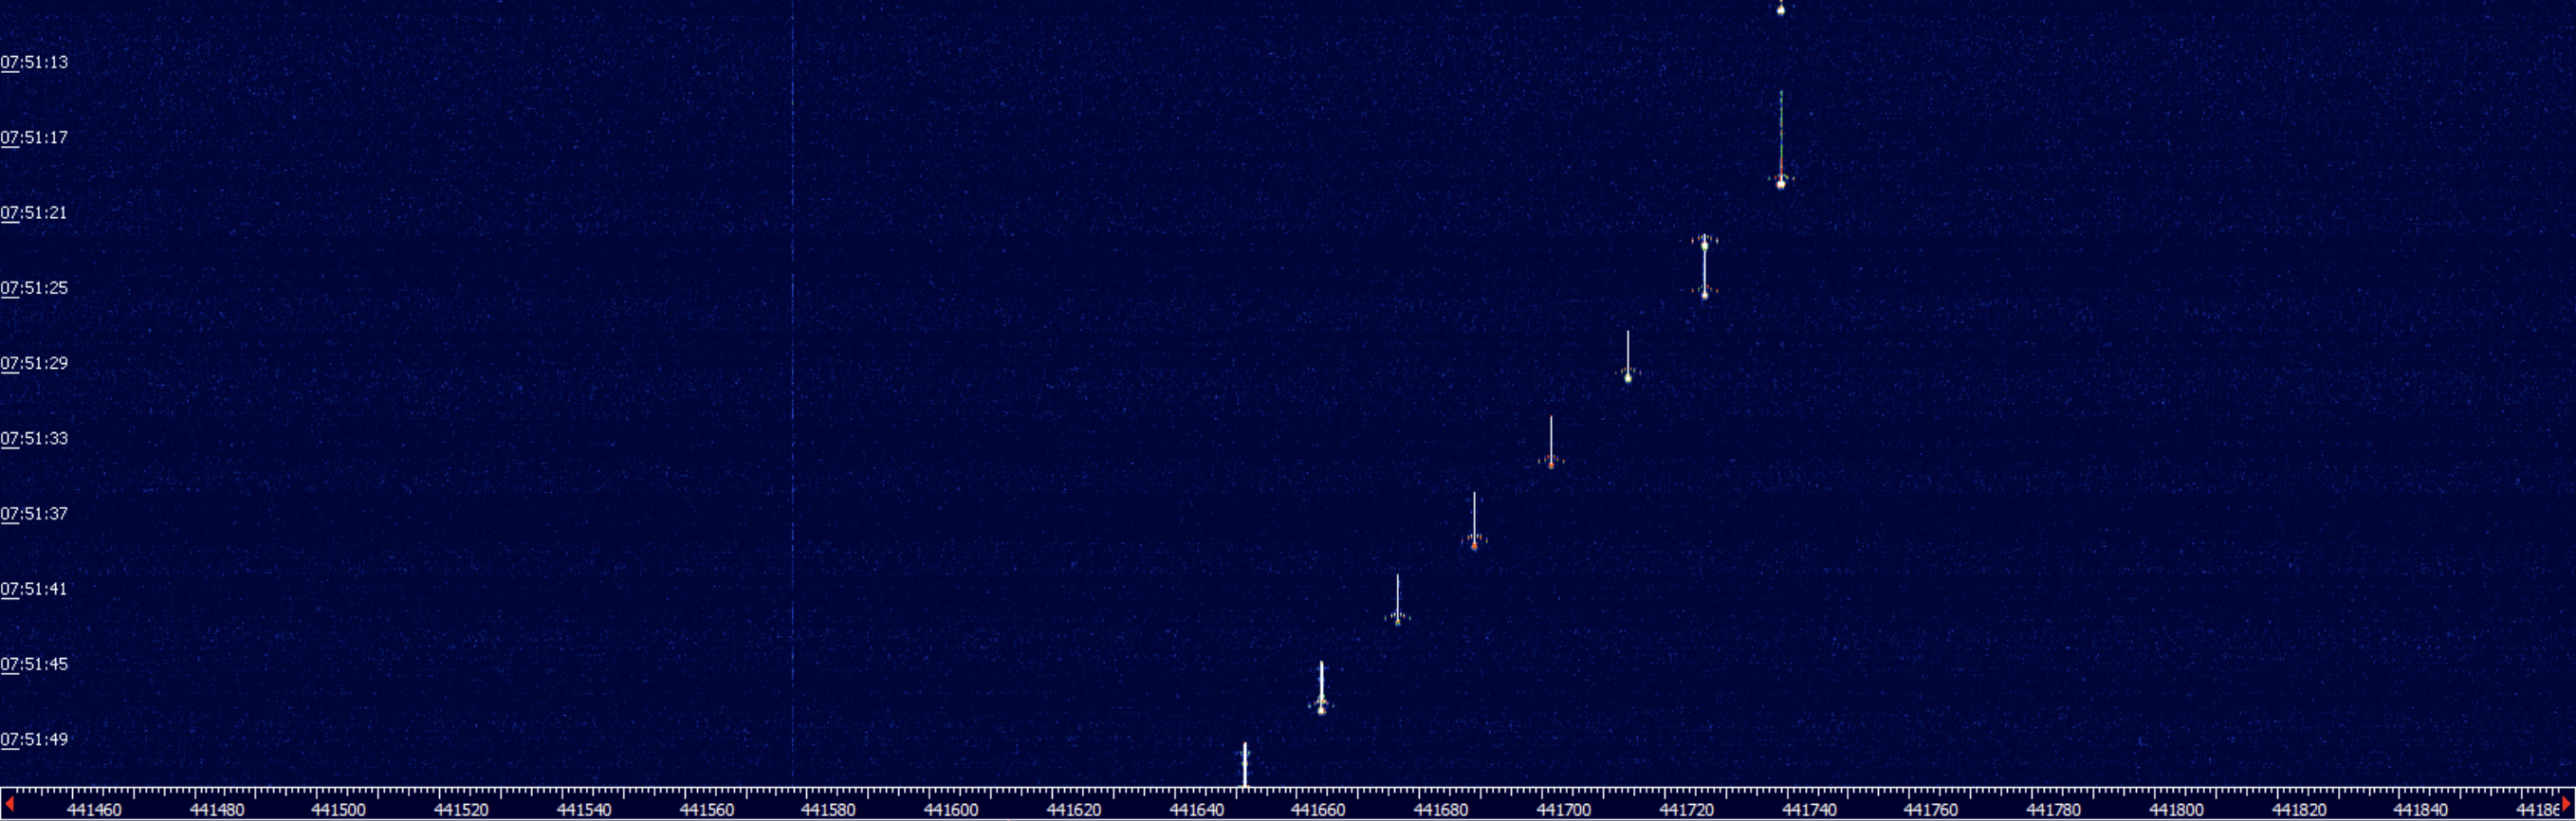
\includegraphics[width=\textwidth]{task3_pmr_445mhz.png}
        \caption{Walkie-talkie stepping through channels 1--8
                 (\SIrange{441.46}{441.84}{\mega\hertz}).}
        \label{fig:pmr}
    \end{subfigure}
    \caption{HDSDR spectra of received radio signals.}
    \label{fig:radio}
\end{figure}

% ------------------------------------------------------------------
\subsection{Task 4 -- Dispersion Curves of DPPH}
% ------------------------------------------------------------------
The dispersion curves of the DPPH samples (\SI{1}{\micro\gram} and
\SI{10}{\micro\gram}) were recorded with the direct-mixing LNB while sweeping the
magnetic field (Section~\ref{sec:sweep}). The characteristic S-shaped dispersion
signal near the LNB output frequency of $\approx \SI{800}{\mega\hertz}$ is clearly
visible (Figure~\ref{fig:dpph}). The resonance field $B_0$ is read off at the
centre of the dispersion feature.

\begin{figure}[H]
    \centering
    \begin{subfigure}{0.48\textwidth}
        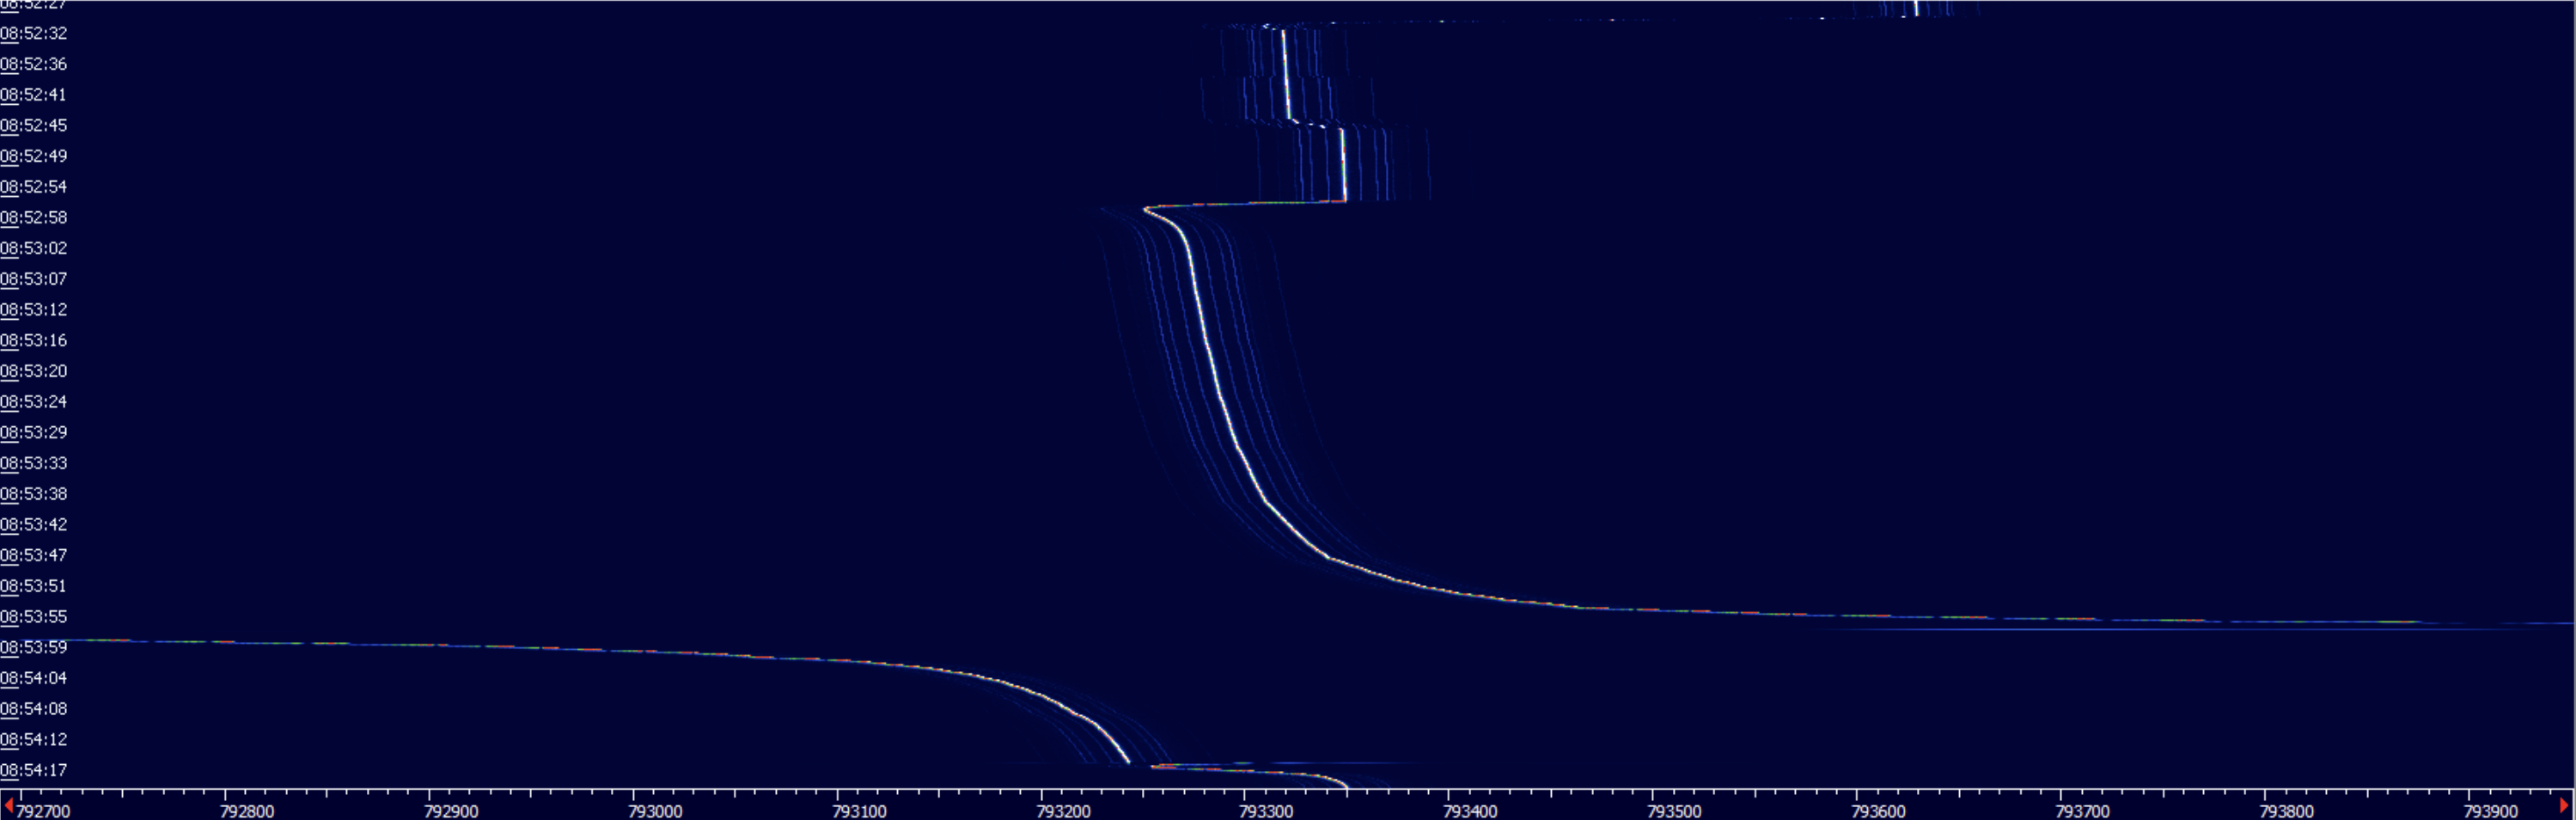
\includegraphics[width=\textwidth]{task4_dpph_1ug.png}
        \caption{DPPH, \SI{1}{\micro\gram}.}
        \label{fig:dpph1}
    \end{subfigure}\hfill
    \begin{subfigure}{0.48\textwidth}
        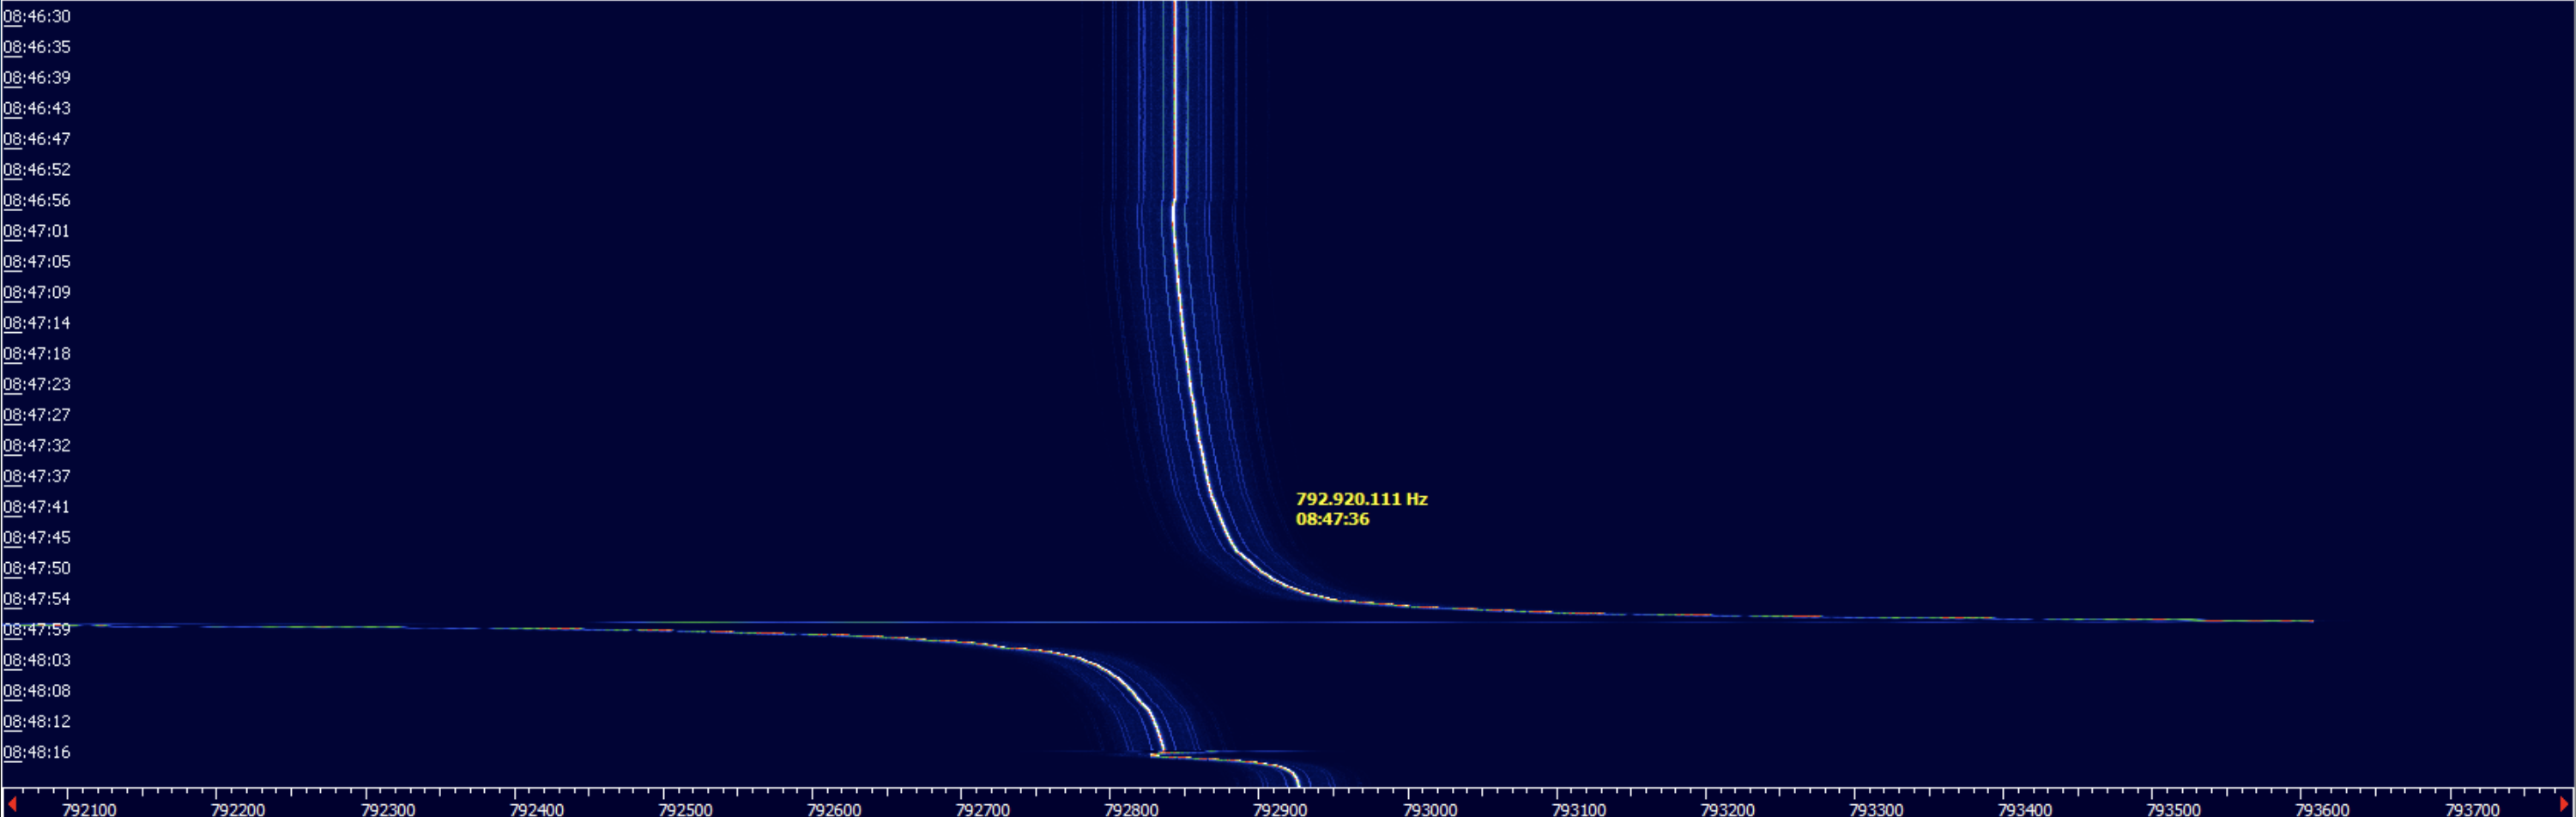
\includegraphics[width=\textwidth]{task4_dpph_10ug.png}
        \caption{DPPH, \SI{10}{\micro\gram}.}
        \label{fig:dpph10}
    \end{subfigure}
    \caption{Dispersion signals of the DPPH samples (HDSDR).}
    \label{fig:dpph}
\end{figure}

Following Section~\ref{sec:processing}, the down-converted frequency was plotted
against the calibrated magnetic flux density $B_0$ for both samples
(Figure~\ref{fig:dpph-curve}); the resonance field is marked by the steepest
point of the S-shaped dispersion feature.

\begin{figure}[H]
    \centering
    \begin{subfigure}{0.48\textwidth}
        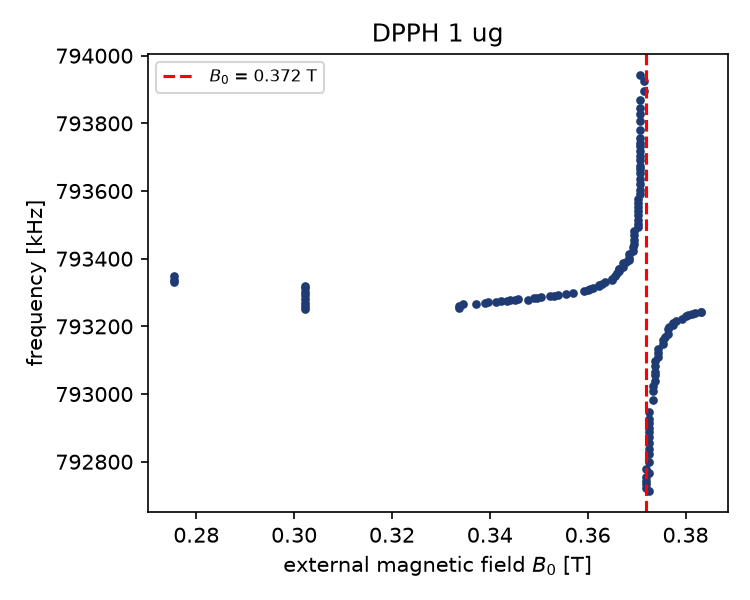
\includegraphics[width=\textwidth]{task4_dpph_1ug_curve.png}
        \caption{DPPH, \SI{1}{\micro\gram}: $B_0 = \SI{0.372}{\tesla}$.}
    \end{subfigure}\hfill
    \begin{subfigure}{0.48\textwidth}
        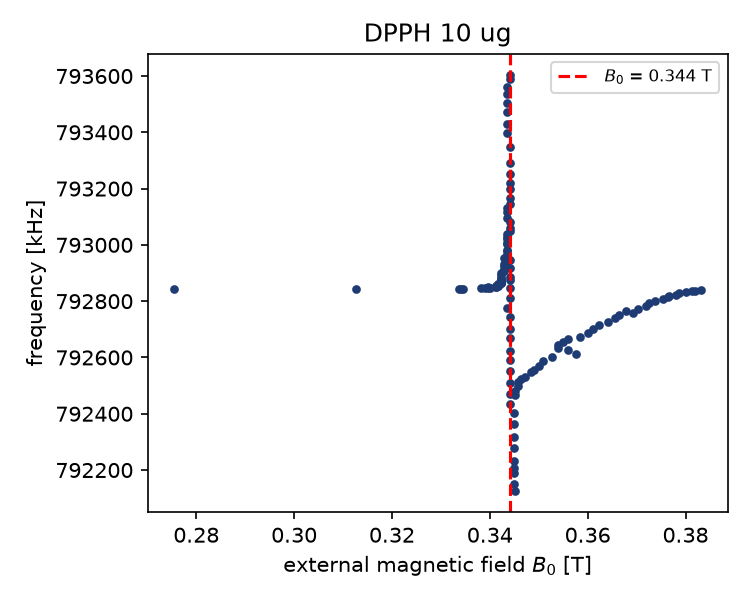
\includegraphics[width=\textwidth]{task4_dpph_10ug_curve.png}
        \caption{DPPH, \SI{10}{\micro\gram}: $B_0 = \SI{0.345}{\tesla}$.}
    \end{subfigure}
    \caption{Down-converted frequency versus calibrated magnetic flux density
             for the DPPH samples, with the resonance field $B_0$ marked
             (dashed line).}
    \label{fig:dpph-curve}
\end{figure}

Inserting the resonance fields $B_0$ together with the nominal LNB coupling
frequency $\nu_0 = \SI{10.6}{\giga\hertz}$ into Equation~\eqref{eq:gfactor}
gives the experimental $g$-factors listed in Table~\ref{tab:dpph}.

\begin{table}[ht]
    \centering
    \caption{Resonance field and $g$-factor of the DPPH samples
             ($\nu_0 = \SI{10.6}{\giga\hertz}$).}
    \label{tab:dpph}
    \begin{tabular}{lccccc}
        \toprule
        Sample & $B_0$ & $g$ (exp.) & $g$ (theo.) & rel.\ error \\
        \midrule
        DPPH \SI{1}{\micro\gram}  & \SI{0.372}{\tesla} & 2.036 & 2.0036 & +1.6\% \\
        DPPH \SI{10}{\micro\gram} & \SI{0.345}{\tesla} & 2.196 & 2.0036 & +9.6\% \\
        \bottomrule
    \end{tabular}
\end{table}

Both experimental $g$-factors come out slightly above the free-radical value of
DPPH, with the \SI{10}{\micro\gram} sample showing a noticeably larger
deviation than the \SI{1}{\micro\gram} sample. This mirrors the systematic
trend reported for this experiment: the larger amount of DPPH increases the
sample's own dipolar broadening / interaction, which shifts the apparent
resonance field slightly and increases the error in the $g$-factor. The
dominant source of the remaining uncertainty, however, is the field
calibration itself (Section~\ref{sec:calibration}): the voltage-to-field
relation was interpolated from a single, video-digitised calibration run with
$\SI{0.05}{\volt}$ steps, so a small misalignment between a calibration step
and the corresponding point of the dispersion sweep translates directly into
an error of several \si{\milli\tesla} in $B_0$ -- and, since
$g \propto 1/B_0$, into a comparable relative error in $g$.

% ------------------------------------------------------------------
\subsection{Task 5 -- Dispersion Curves of Ultramarine}
% ------------------------------------------------------------------
The dispersion curves of the Ultramarine samples were measured at the dilution
levels pure (undiluted), 1:10, 1:100 and 1:1000
(Figure~\ref{fig:um}). With increasing dilution the amount of paramagnetic
material -- and therefore the signal amplitude -- decreases.

\begin{figure}[H]
    \centering
    \begin{subfigure}{0.48\textwidth}
        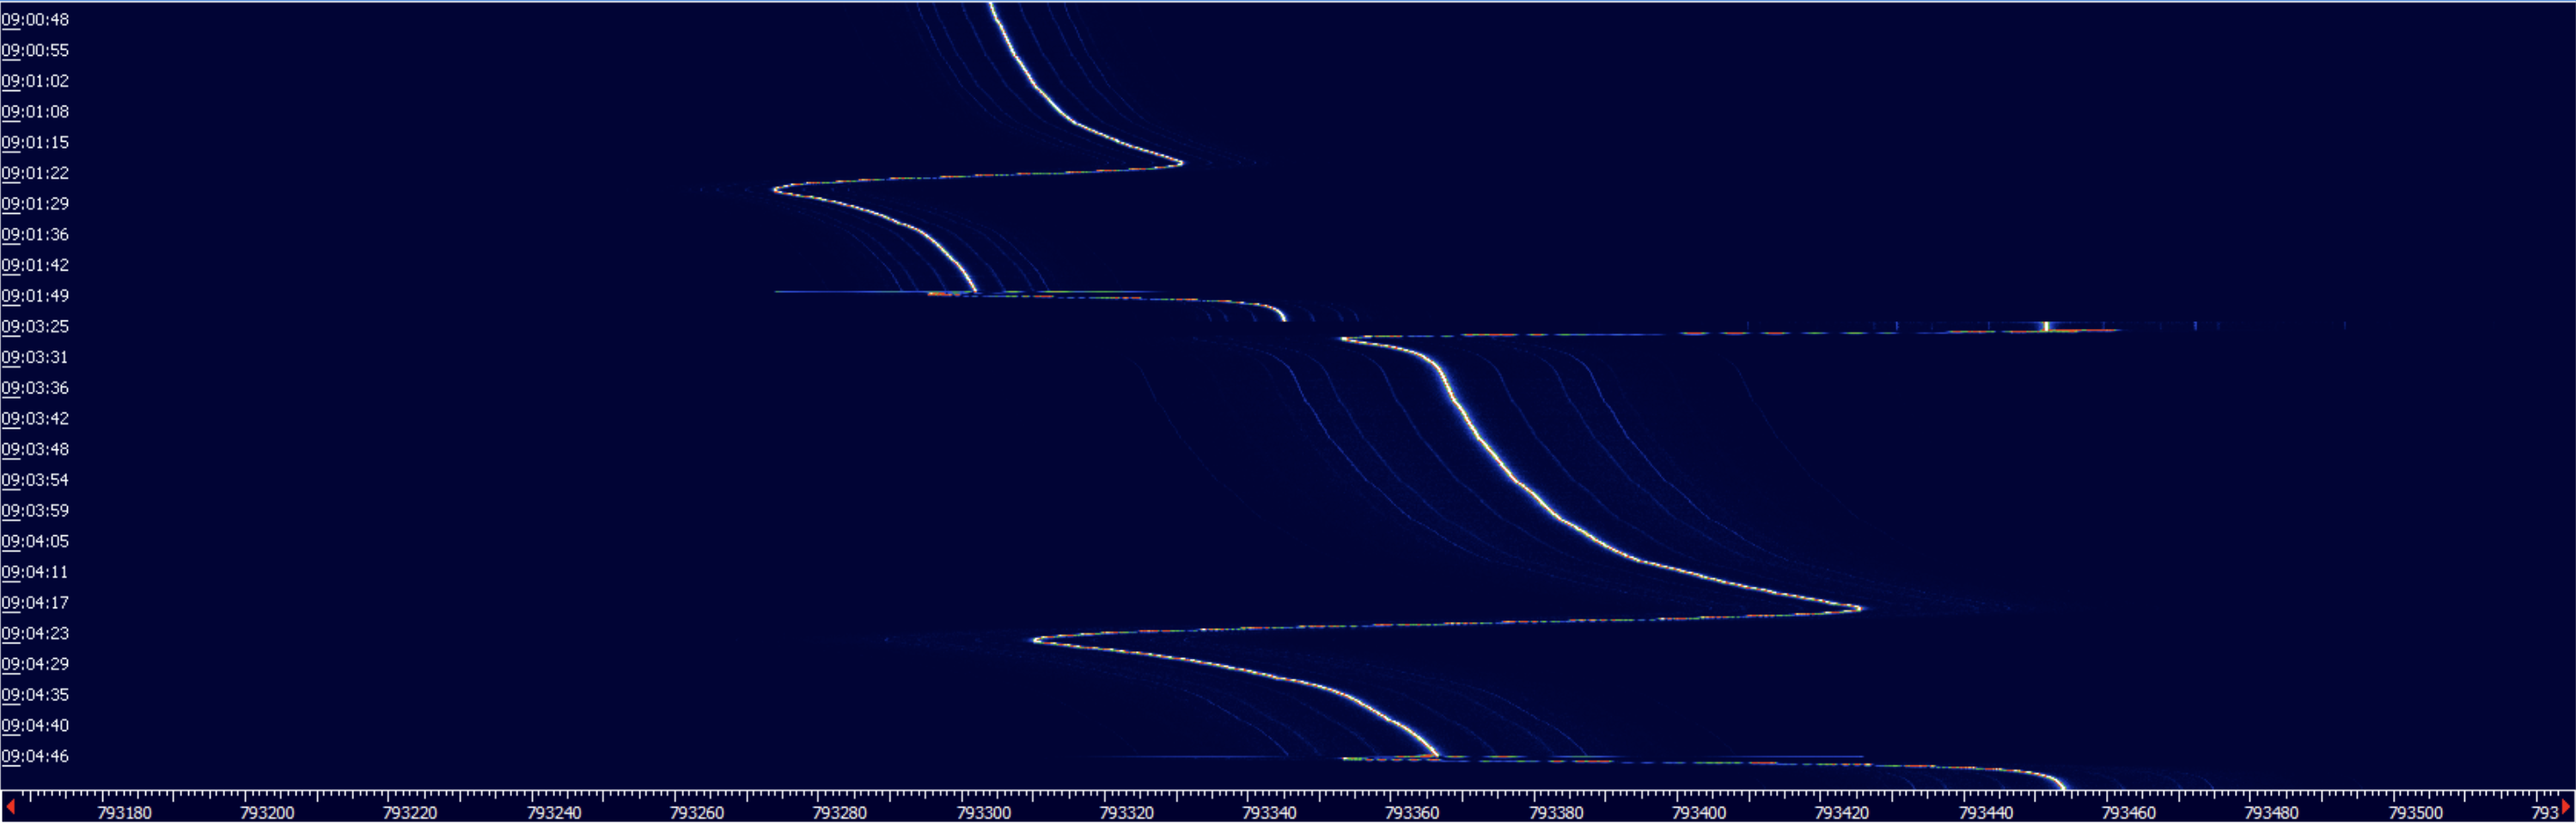
\includegraphics[width=\textwidth]{task5_um_pure.png}
        \caption{Pure (undiluted).}
    \end{subfigure}\hfill
    \begin{subfigure}{0.48\textwidth}
        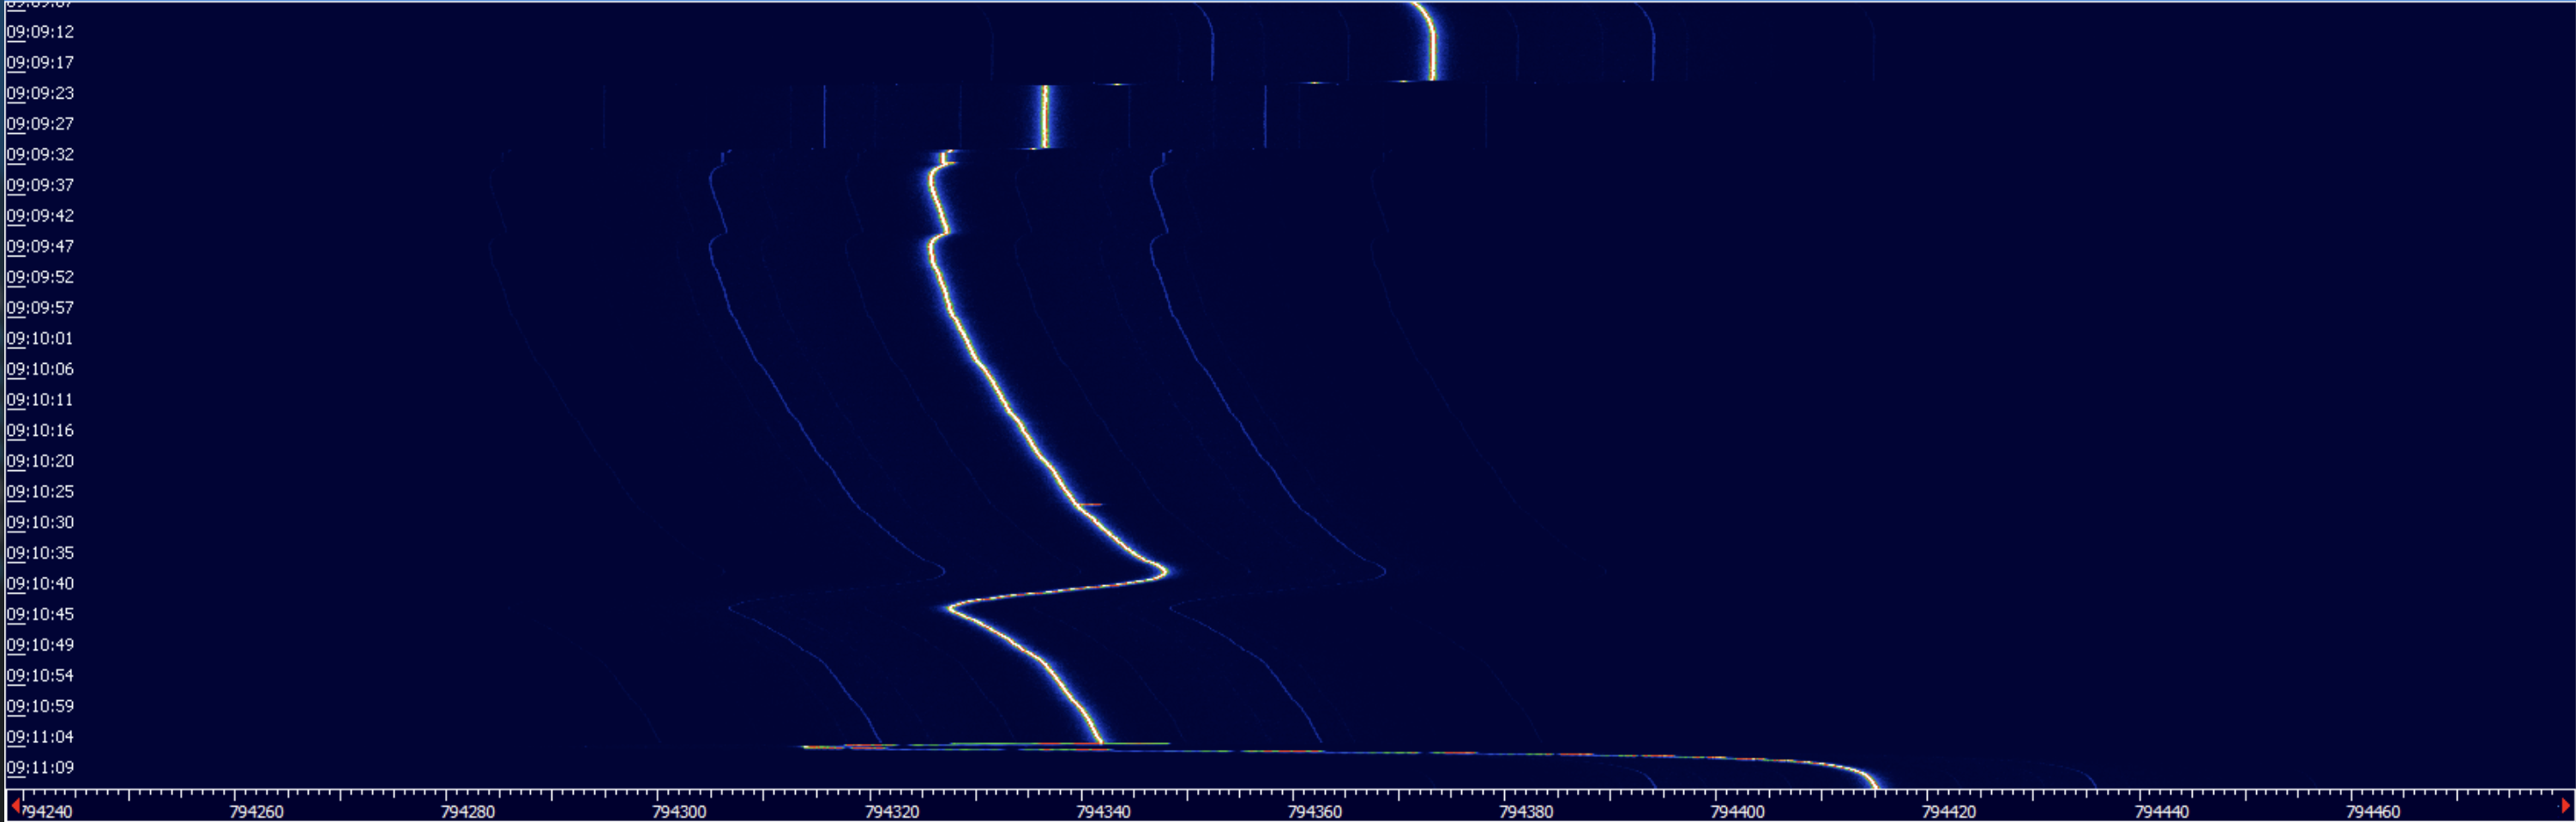
\includegraphics[width=\textwidth]{task5_um_1_10.png}
        \caption{1:10.}
    \end{subfigure}

    \vspace{0.4cm}
    \begin{subfigure}{0.48\textwidth}
        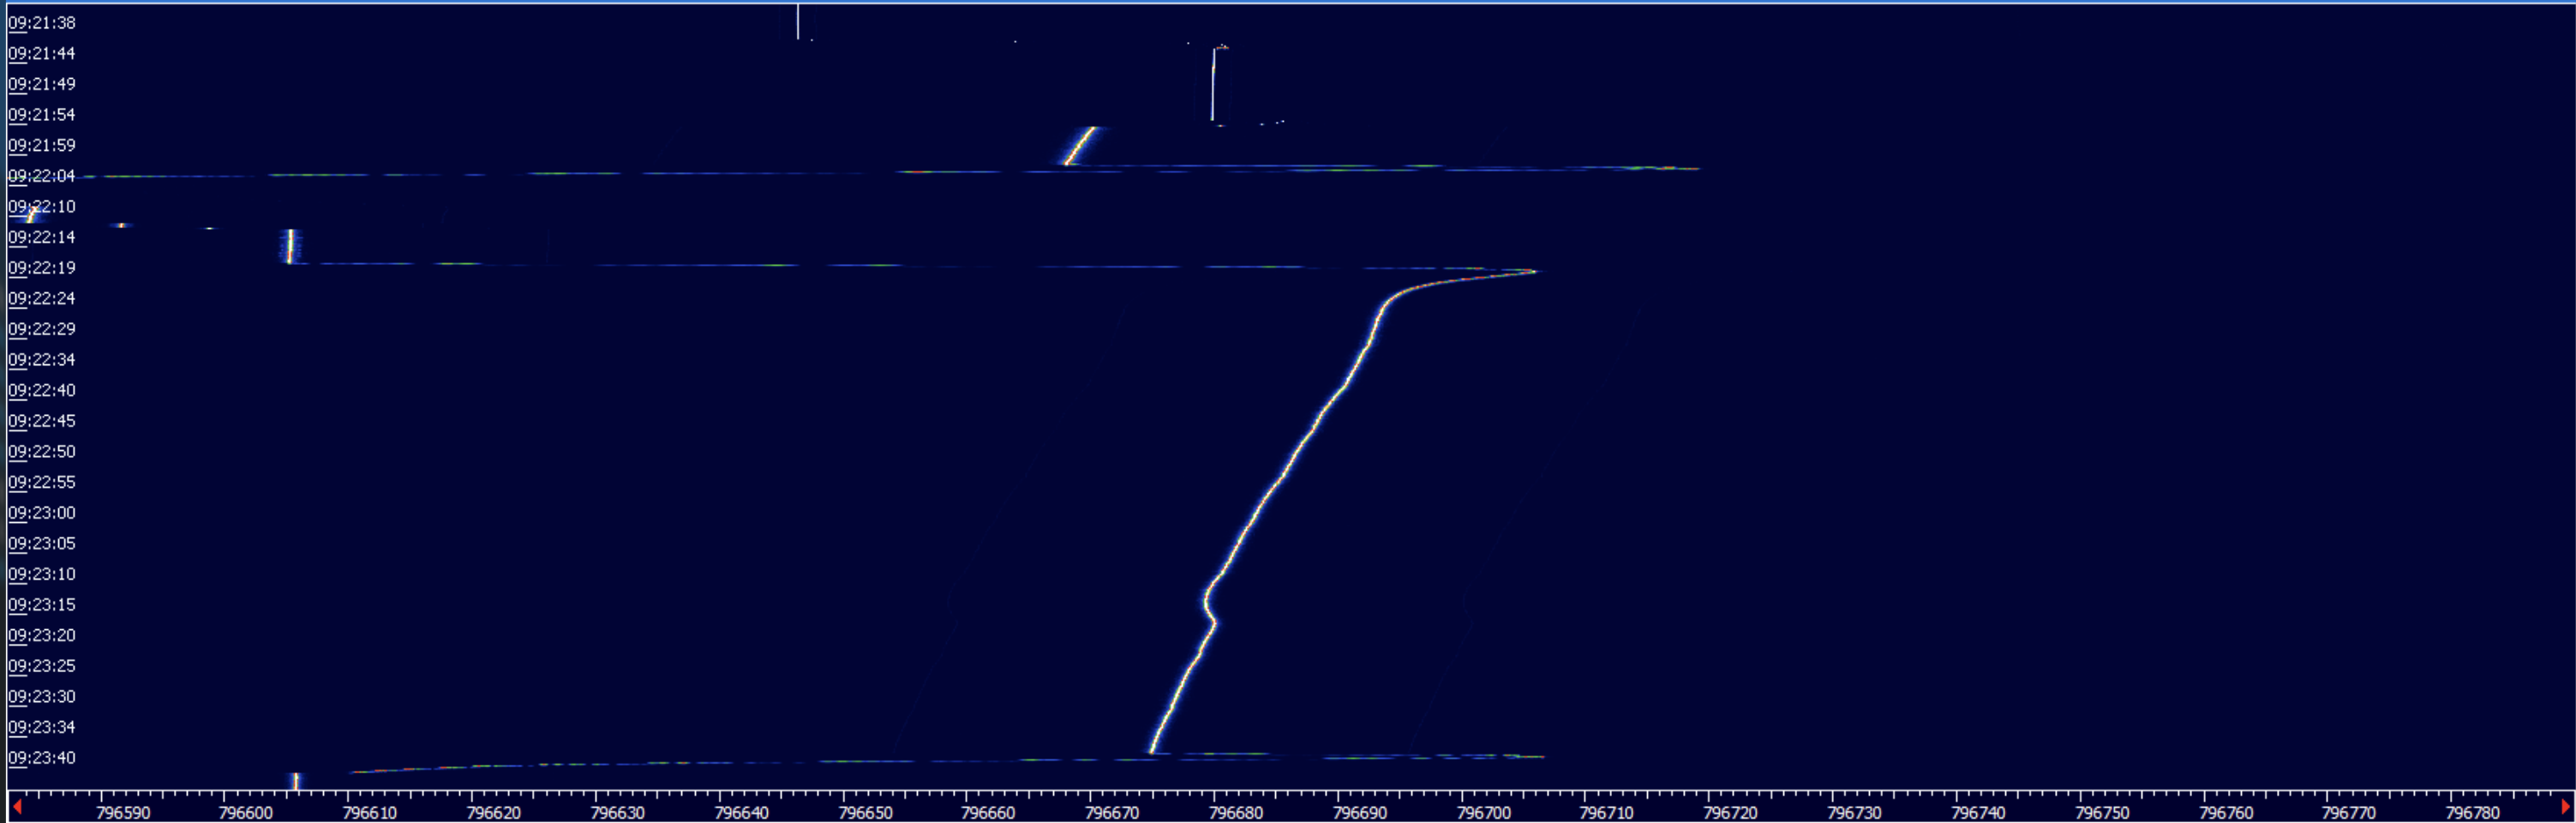
\includegraphics[width=\textwidth]{task5_um_1_100.png}
        \caption{1:100.}
    \end{subfigure}\hfill
    \begin{subfigure}{0.48\textwidth}
        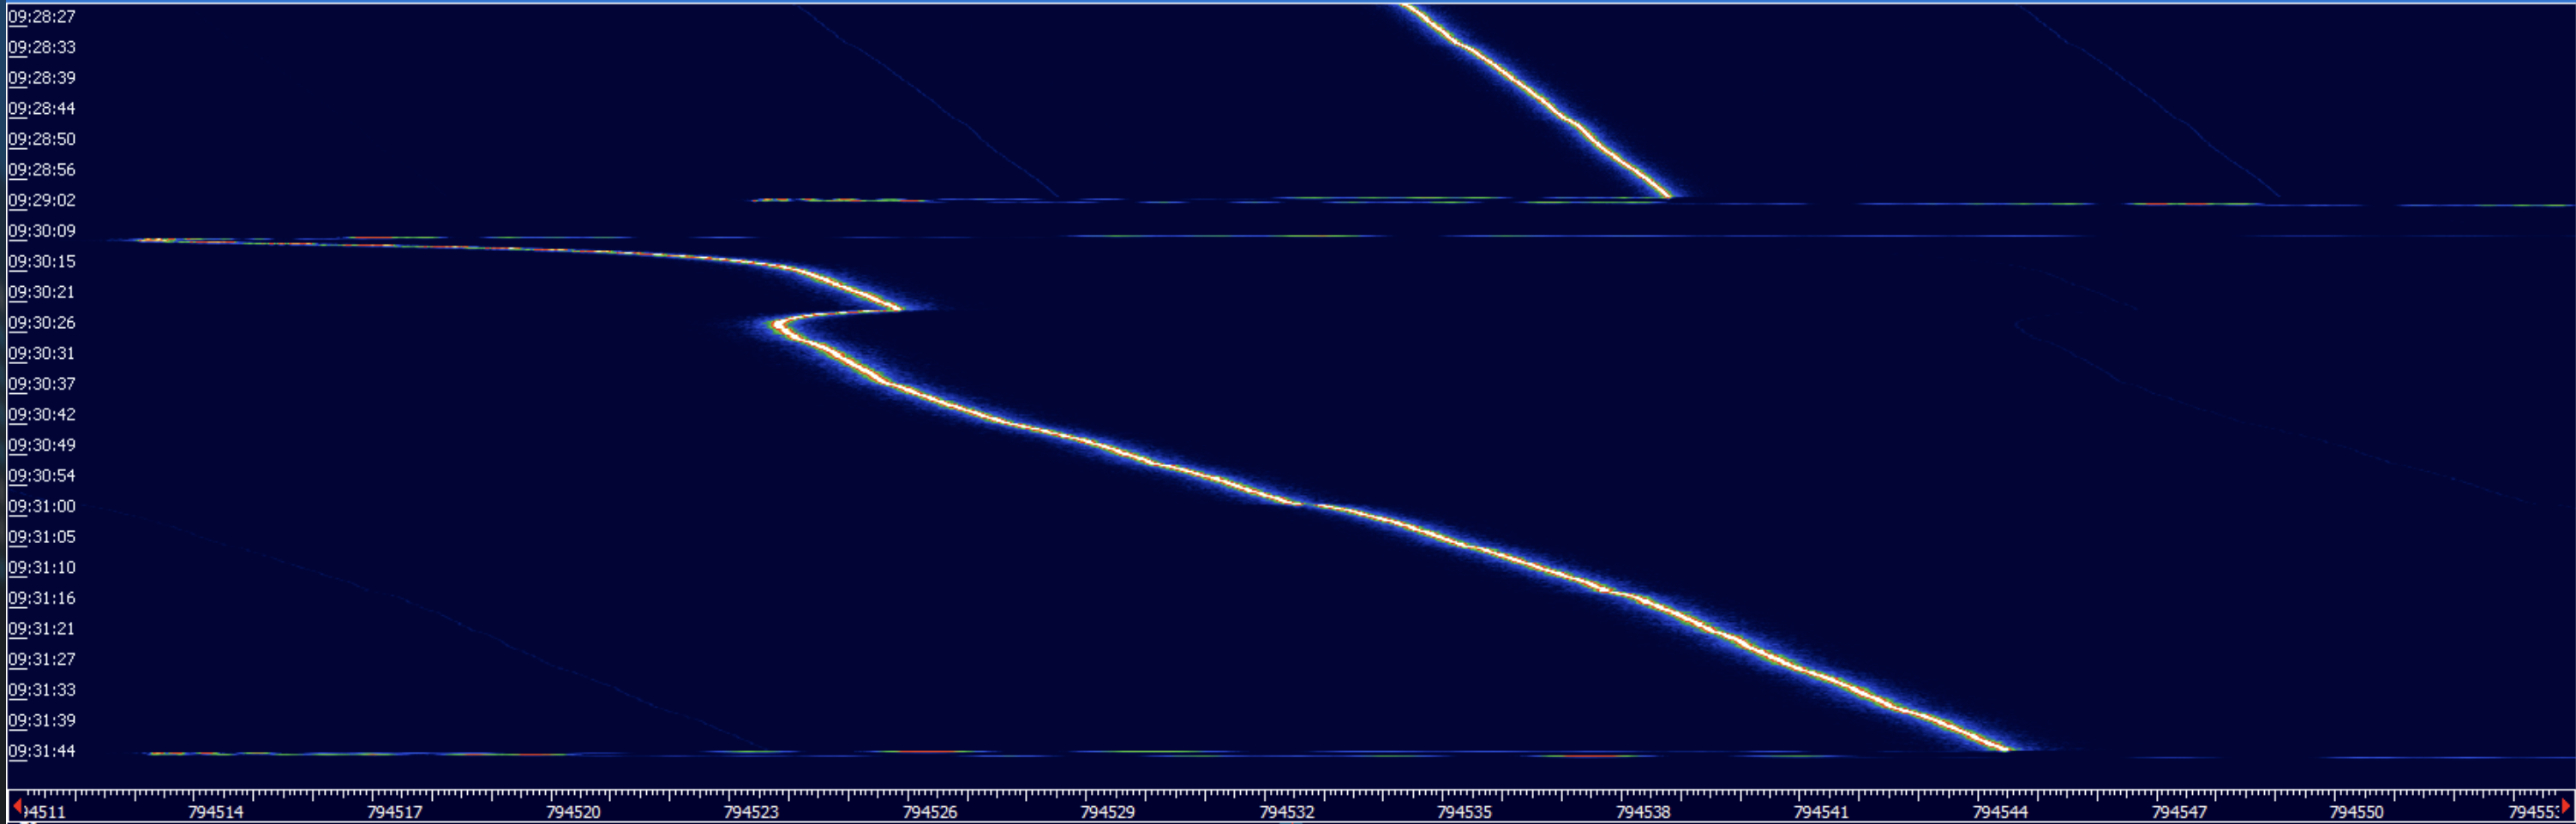
\includegraphics[width=\textwidth]{task5_um_1_1000.png}
        \caption{1:1000.}
    \end{subfigure}
    \caption{Dispersion signals of the Ultramarine samples at different dilution
             levels (HDSDR).}
    \label{fig:um}
\end{figure}

As for the DPPH samples (Section~\ref{sec:processing}), the down-converted
frequency was plotted against the calibrated magnetic flux density $B_0$ for
all four dilution levels (Figure~\ref{fig:um-curve}). The dispersion feature
is clearly S-shaped and sharp for the undiluted sample and the 1:10 dilution.
For the more diluted 1:100 and 1:1000 samples it is much weaker and sits on
top of a pronounced slow drift of the down-converted frequency across the
sweep; only after subtracting this drift (Section~\ref{sec:processing}) does
the underlying S-shaped feature become visible.

\begin{figure}[H]
    \centering
    \begin{subfigure}{0.48\textwidth}
        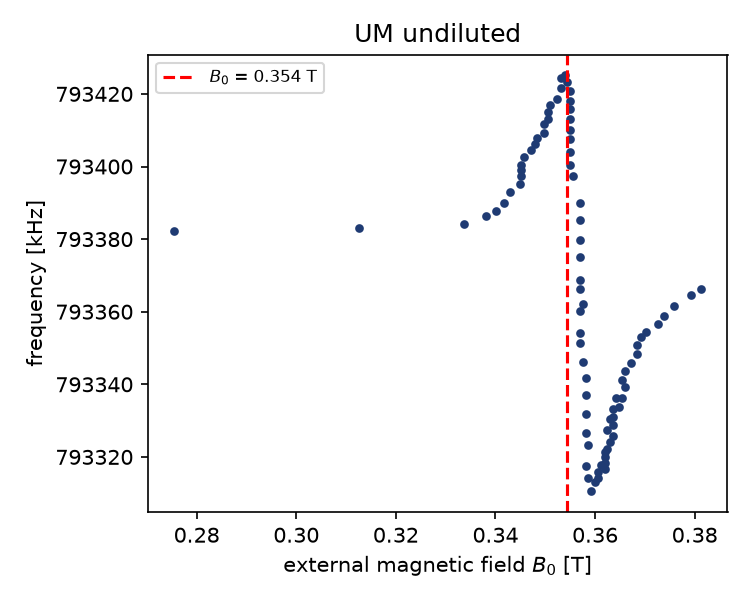
\includegraphics[width=\textwidth]{task5_um_pure_curve.png}
        \caption{Pure (undiluted): $B_0 = \SI{0.354}{\tesla}$.}
    \end{subfigure}\hfill
    \begin{subfigure}{0.48\textwidth}
        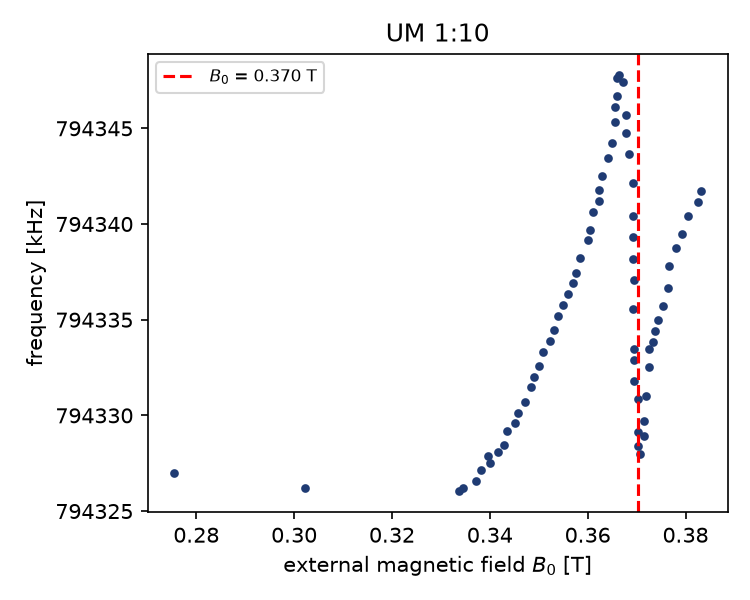
\includegraphics[width=\textwidth]{task5_um_1_10_curve.png}
        \caption{1:10: $B_0 = \SI{0.370}{\tesla}$.}
    \end{subfigure}

    \vspace{0.4cm}
    \begin{subfigure}{0.48\textwidth}
        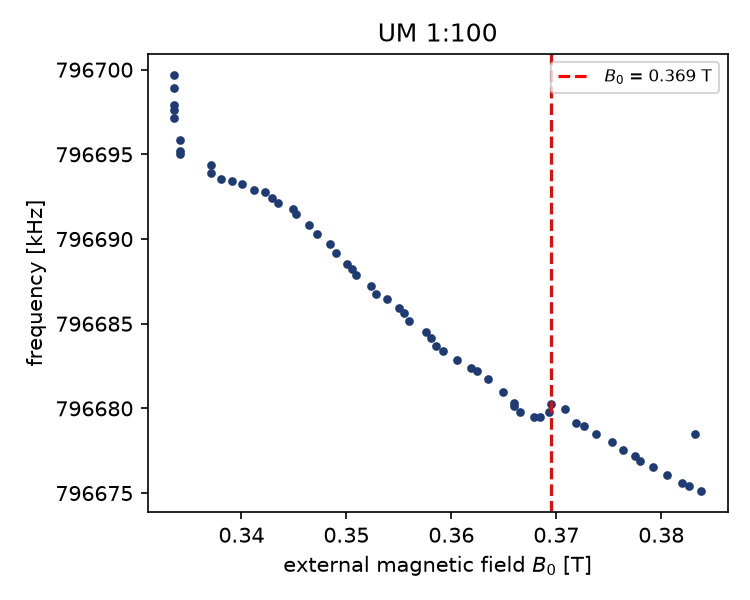
\includegraphics[width=\textwidth]{task5_um_1_100_curve.png}
        \caption{1:100: $B_0 = \SI{0.370}{\tesla}$.}
    \end{subfigure}\hfill
    \begin{subfigure}{0.48\textwidth}
        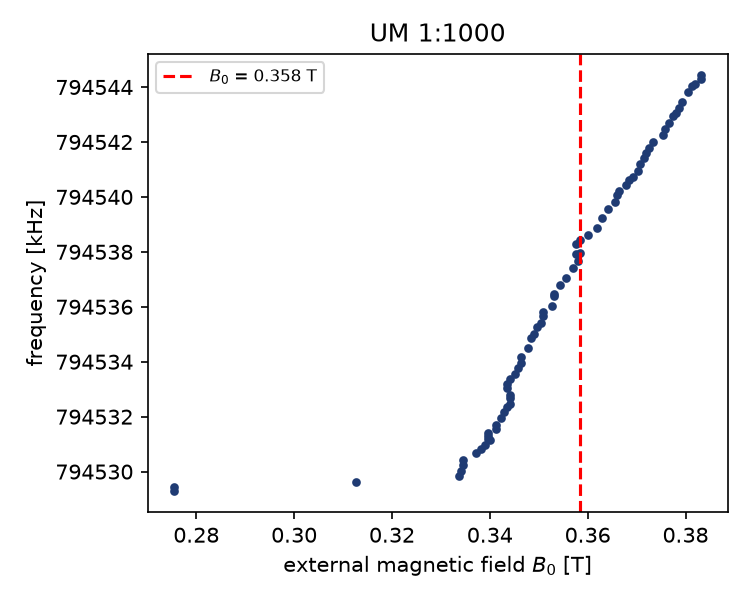
\includegraphics[width=\textwidth]{task5_um_1_1000_curve.png}
        \caption{1:1000: $B_0 = \SI{0.359}{\tesla}$.}
    \end{subfigure}
    \caption{Down-converted frequency versus calibrated magnetic flux density
             for the Ultramarine samples, with the resonance field $B_0$
             marked (dashed line). For the two most diluted samples the mark
             sits on a small residual feature riding on top of a slow drift
             of the baseline frequency (see text).}
    \label{fig:um-curve}
\end{figure}

\begin{table}[ht]
    \centering
    \caption{Resonance field and $g$-factor of the Ultramarine samples
             ($\nu_0 = \SI{10.6}{\giga\hertz}$).}
    \label{tab:um}
    \begin{tabular}{lccccc}
        \toprule
        Sample & $B_0$ & $g$ (exp.) & $g$ (theo.) & rel.\ error \\
        \midrule
        Undiluted & \SI{0.354}{\tesla} & 2.137 & 2.0290 & +5.3\% \\
        1:10      & \SI{0.370}{\tesla} & 2.045 & 2.0290 & +0.8\% \\
        1:100     & \SI{0.370}{\tesla} & 2.050 & 2.0290 & +1.0\% \\
        1:1000    & \SI{0.359}{\tesla} & 2.113 & 2.0290 & +4.1\% \\
        \bottomrule
    \end{tabular}
\end{table}

The 1:10 and 1:100 dilutions give the smallest deviation from the literature
value, while the undiluted sample shows the largest error. This is a
different ranking than a naive reading of Figure~\ref{fig:um} would suggest
(the undiluted sample has by far the strongest raw signal): once the slow
baseline drift is removed, the residual dispersion feature of the 1:100
sample turns out to be just as sharp and well-defined as that of the
strongest samples (Figure~\ref{fig:um-curve}), whereas the undiluted sample's
resonance sits on the steep flank of its own S-curve, making the exact
field of steepest slope more sensitive to the local point spacing. There is
consequently no monotonic trend of the error with dilution: the sharpness of
the (drift-corrected) dispersion feature depends on a combination of the
remaining sample concentration and how closely the fixed field sweep happened
to bracket the resonance, not on dilution alone. As with DPPH, the field calibration
(Section~\ref{sec:calibration}) remains the main source of systematic
uncertainty in $B_0$ and therefore in $g$.

% ------------------------------------------------------------------
\subsection{Task 6 -- DPPH \texorpdfstring{\SI{10}{\micro\gram}}{10 ug} with a Calibrated LNB}
% ------------------------------------------------------------------
The \SI{10}{\micro\gram} DPPH sample was measured again, this time with a
calibrated PLL LNB (single LO at exactly \SI{9.75}{\giga\hertz}) as the
observation system (Figure~\ref{fig:task6}). The resonance frequency and the
resulting $g$-factor are compared with the value obtained by the direct mixing
method in Task~4 to assess the accuracy of the magnetic-flux-density display.
The photographed dispersion curve was processed exactly as in
Section~\ref{sec:processing}: the last \SI{80}{\second} of the sweep before
the final (temporally last) digitised point were assigned the corresponding
\SIrange{26}{30}{\volt} voltage ramp and converted to $B_0$ via the
calibration of Section~\ref{sec:calibration}, this time using the exactly
known LO frequency $\nu_0 = \SI{9.75}{\giga\hertz}$ in
Equation~\eqref{eq:gfactor}.

\begin{figure}[H]
    \centering
    \begin{subfigure}{0.48\textwidth}
        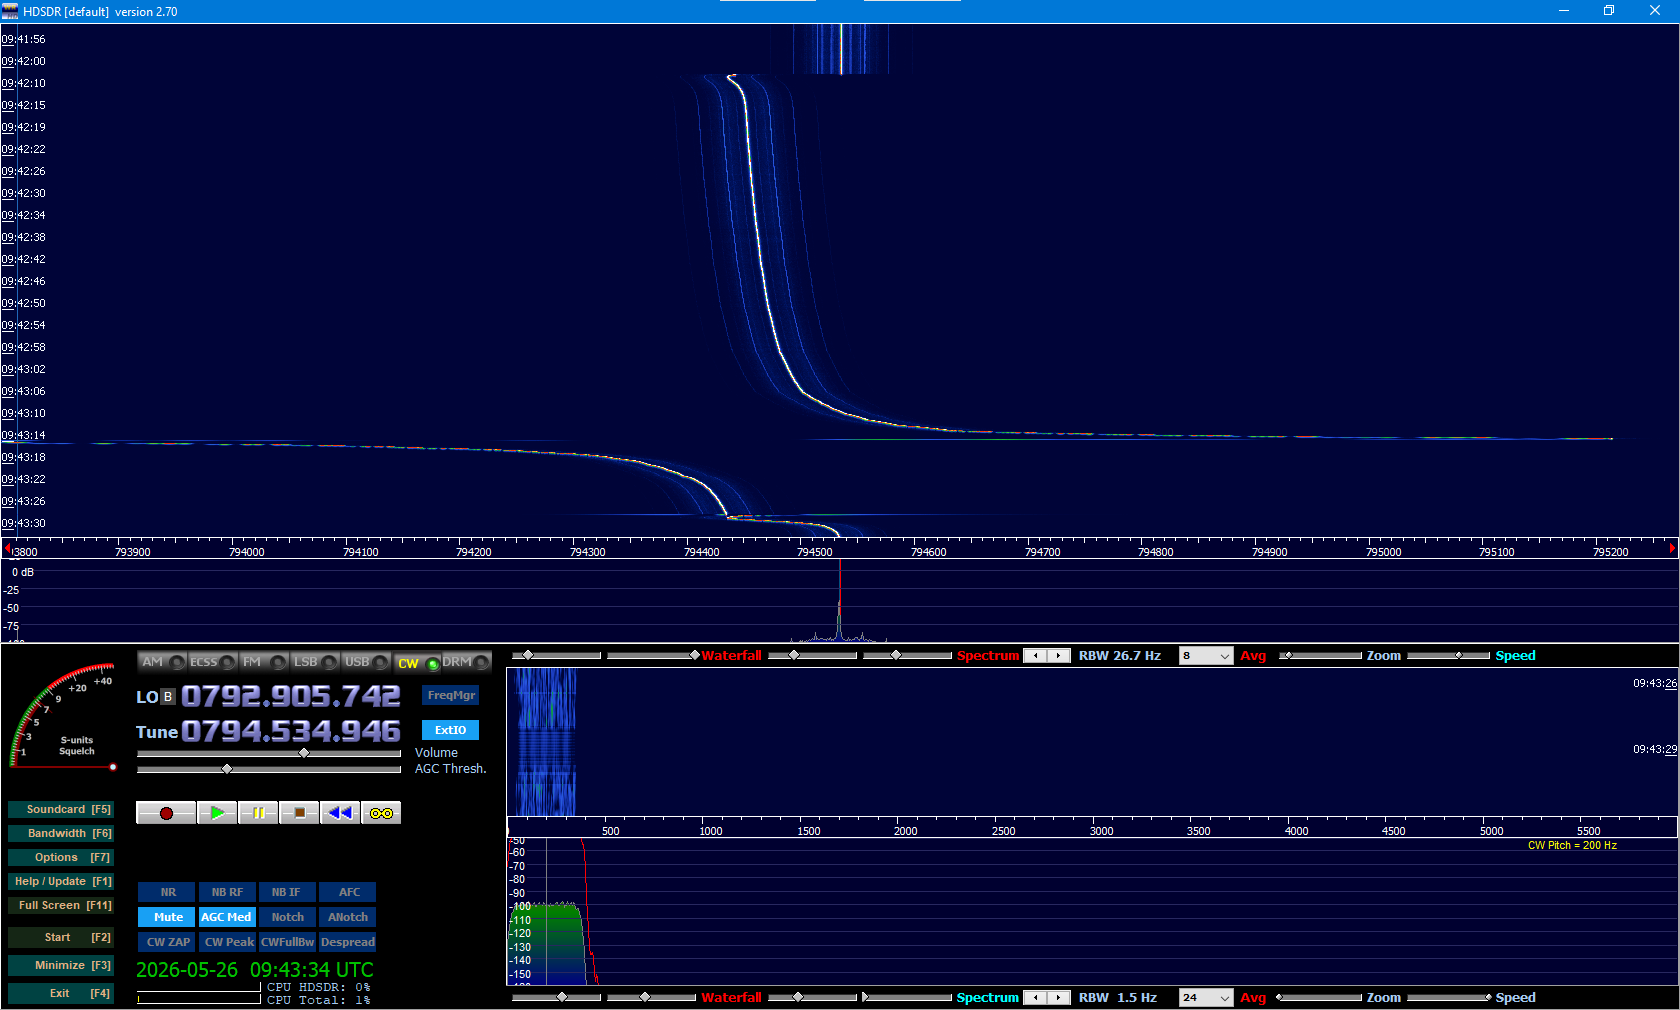
\includegraphics[width=\textwidth]{task6_dpph_calibrated.png}
        \caption{Dispersion signal (HDSDR).}
    \end{subfigure}\hfill
    \begin{subfigure}{0.48\textwidth}
        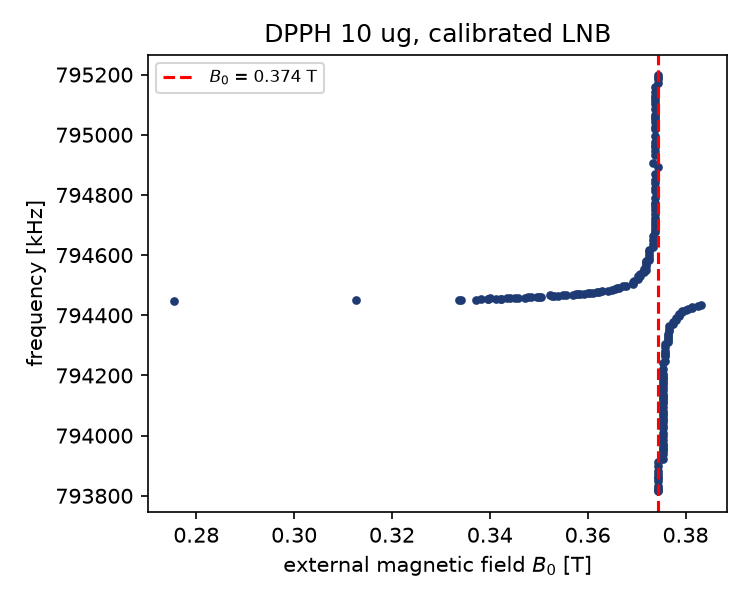
\includegraphics[width=\textwidth]{task6_dpph_calibrated_curve.png}
        \caption{Digitised curve, $B_0 = \SI{0.374}{\tesla}$.}
    \end{subfigure}
    \caption{Dispersion signal of DPPH \SI{10}{\micro\gram} measured with the
             calibrated PLL LNB, and the resulting down-converted frequency
             versus calibrated magnetic flux density.}
    \label{fig:task6}
\end{figure}

\begin{table}[ht]
    \centering
    \caption{Comparison of the DPPH \SI{10}{\micro\gram} measurement with the
             uncalibrated (Task~4) and the calibrated (Task~6) LNB.}
    \label{tab:task6}
    \begin{tabular}{lccc}
        \toprule
         & Task 4 (uncalibrated) & Task 6 (calibrated) & Change \\
        \midrule
        $\nu_0$   & \SI{10.6}{\giga\hertz} (assumed) & \SI{9.75}{\giga\hertz} (exact) & -- \\
        $B_0$     & \SI{0.345}{\tesla} & \SI{0.374}{\tesla} & \SI{+29}{\milli\tesla} \\
        $g$ (exp.)& 2.196 & 1.861 & $-15.3\%$ \\
        rel.\ error & $+9.6\%$ & $-7.1\%$ & -- \\
        \bottomrule
    \end{tabular}
\end{table}

Both measurements deviate from the literature value $g = 2.0036$ by a
comparable magnitude ($\approx \SI{10}{\percent}$), but in opposite
directions: the uncalibrated LNB (assumed $\nu_0 = \SI{10.6}{\giga\hertz}$)
overestimates $g$, while the calibrated LNB (exact $\nu_0 =
\SI{9.75}{\giga\hertz}$) underestimates it. Since $g \propto \nu_0/B_0$, this
sign flip cannot be explained by the change in $\nu_0$ alone -- reducing
$\nu_0$ from \SI{10.6}{} to \SI{9.75}{\giga\hertz} (a factor $0.92$) would, at
the same $B_0$, simply scale $g$ down by the same factor. Instead, the
resonance field itself came out \SI{29}{\milli\tesla} higher in Task~6
($\SI{0.374}{\tesla}$ vs.\ $\SI{0.345}{\tesla}$), which more than compensates
the lower $\nu_0$. Because both sweeps were digitised from independent
photographs and mapped onto the calibration curve independently, this
indicates that the main source of error is still the magnetic field
calibration (Section~\ref{sec:calibration}) rather than the LNB frequency:
knowing $\nu_0$ exactly in Task~6 removes one source of uncertainty, but the
\si{\milli\tesla}-level accuracy of the video-based $B_0$ calibration remains
the limiting factor for the $g$-factor in both tasks.

% ==================================================================
\section{Conclusion}
% ==================================================================
Task~1 confirmed the expected sum and difference frequencies of a mixed RF
signal, and Tasks~2/3 demonstrated reception of VLF, FM and PMR signals with
the RSP1/HDSDR system. For the EPR measurements (Tasks~4 and~5), the
dispersion curves of the DPPH and Ultramarine samples all show the
characteristic S-shaped feature of a dispersive resonance line, and the
resulting $g$-factors (Tables~\ref{tab:dpph} and~\ref{tab:um}) lie within
roughly \SIrange{1}{10}{\percent} of the literature values ($g_{\text{DPPH}} =
2.0036$, $g_{\text{UM}} = 2.0290$), which is a reasonable agreement given the
uncalibrated LNB frequency ($\nu_0 \approx \SI{10.6}{\giga\hertz}$, not
independently measured) and the resolution of the video-based field
calibration. No strict monotonic trend between sample concentration/dilution
and the error in $g$ was found; after correcting for the slow baseline drift
of the down-converted frequency (Section~\ref{sec:processing}), even the
weakly paramagnetic UM 1:100 sample yields one of the best agreements with
theory. The largest deviations instead occur for DPPH \SI{10}{\micro\gram}
and the undiluted UM sample, where the resonance sits on the steep flank of a
very sharp S-curve, making the point of steepest slope more sensitive to the
exact sample spacing, while the sharply and cleanly resolved DPPH
\SI{1}{\micro\gram} and UM 1:10 / 1:100 curves give the best agreement with
theory.

The main systematic uncertainty in all $g$-factors is the magnetic field
calibration (Section~\ref{sec:calibration}): the field was not measured
directly during the dispersion sweeps but reconstructed from the programmed
supply voltage via a single video-digitised calibration curve, so the
accuracy of $B_0$ is ultimately limited by how well that calibration
represents the true field at each voltage step. Task~6 confirms this: even
with the LO frequency of the calibrated PLL LNB known exactly
($\nu_0 = \SI{9.75}{\giga\hertz}$, Table~\ref{tab:task6}), the resulting
$g$-factor for DPPH \SI{10}{\micro\gram} deviates from theory by about the
same amount as the uncalibrated Task~4 measurement, just with the opposite
sign. Eliminating the uncertainty in $\nu_0$ therefore does not by itself
improve the accuracy of $g$ -- the dominant remaining error is the
determination of $B_0$ from the video calibration, not the LNB frequency.

\end{document}
